% =====================================================================
%  report_figures.tex
%  AI-Powered Autonomous Smart Agriculture
%  Population-based Optimization (PSO, GA) + Reinforcement Learning (VI, Q-learning)
%
%  This file embeds every generated figure and explains, in beginner
%  language, exactly what each graph, axis, curve, colour and symbol
%  means.  Compile with pdflatex (run from the project root so the
%  relative image paths outputs/figures/... resolve correctly).
% =====================================================================
\documentclass[11pt]{article}

\usepackage[a4paper,margin=1in]{geometry}
\usepackage{graphicx}
\usepackage{float}          % the [H] float placement
\usepackage{booktabs}       % nice tables
\usepackage{amsmath}
\usepackage{amssymb}        % \bigstar, \blacksquare, etc.
\usepackage{enumitem}       % tight itemize/description lists
\usepackage{xcolor}
\usepackage{hyperref}

\graphicspath{{outputs/figures/}}

% A small reusable "How to read this figure" block.
\newcommand{\readhead}{\medskip\noindent\textbf{\textcolor{green!45!black}{How to
read this figure:}}\par\nobreak}
\newlist{readlist}{itemize}{1}
\setlist[readlist]{leftmargin=1.5em,itemsep=1.5pt,topsep=2pt,parsep=0pt}

\title{\textbf{AI-Powered Autonomous Smart Agriculture}\\[4pt]
\large Swarm Intelligence and Reinforcement Learning for an\\
Autonomous Pollination System --- Figure Guide}
\author{Department of Computer Science and Engineering, University of Dhaka\\
CSE 4101 -- Artificial Intelligence Laboratory}
\date{\today}

\begin{document}
\maketitle

\begin{abstract}
This document presents and explains every figure produced by the
autonomous pollination system. The system couples two Artificial
Intelligence paradigms. \textbf{Global optimization (Population-based
metaheuristics)} assigns flowers to robots: Particle Swarm Optimization (PSO)
and a Genetic Algorithm (GA) are compared for allocation on an identical
environment and fitness function.
\textbf{Sequential decision making (Reinforcement Learning)} then guides a
robot through a grid-world Markov Decision Process (MDP): Value Iteration
(model-based) and Q-learning (model-free) are compared. Every figure is
accompanied by a plain-language ``how to read it'' breakdown of its axes,
curves, colours and symbols.
\end{abstract}

\tableofcontents
\newpage

% =====================================================================
\section{How to Read These Figures (Notation Key)}
% =====================================================================
Before the figures, here is a one-time key to the symbols and words that
recur throughout. Refer back here whenever a symbol is unfamiliar.

\subsection{Markers on the ``map'' and ``grid'' figures}
The allocation maps (Phase~1) and the navigation grids (Phase~2) reuse a fixed
visual vocabulary:
\begin{description}[leftmargin=2.2em,style=nextline,itemsep=2pt,topsep=3pt]
  \item[Coloured dots] Flowers. On the \emph{allocation maps} the colour tells
        you \emph{which robot} is responsible for that flower.
  \item[$\bigstar$ Magenta star] A target flower the robot must reach and
        pollinate (a ``goal'' cell) on the \emph{navigation grids}.
  \item[$\blacksquare$ Black square] An obstacle --- an impassable cell (tree,
        rock, water channel). The robot can never enter it.
  \item[Green/lime square] The robot's \emph{start} cell (its depot / parking
        spot).
  \item[``P'' marker (cyan or lime)] A charging station --- where the robot
        must return once every flower is done.
  \item[Red $\times$] An obstacle on the allocation maps.
  \item[Small grey arrows ($\uparrow\ \downarrow\ \leftarrow\ \rightarrow$)]
        The \emph{policy}: the single best direction to move from that cell.
        A whole field of arrows is a complete strategy for the robot.
  \item[Coloured line with dots] The robot's actual \emph{path} (trajectory)
        as it moves from cell to cell.
\end{description}

\subsection{Symbols and words used in the plots}
\begin{description}[leftmargin=2.2em,style=nextline,itemsep=2pt,topsep=3pt]
  \item[Fitness] A single ``score'' that blends all six allocation objectives
        into one number. It is a \textbf{cost}, so \textbf{lower is better}.
  \item[Coverage] Fraction of flowers actually pollinated ($100\%$ = every
        flower served). Higher is better.
  \item[Total distance] Sum of all robots' flight distances, in metres.
  \item[Energy] Battery units used --- directly proportional to distance.
  \item[Completion time / makespan] The moment the \emph{last} (slowest) robot
        finishes; the fleet is only done when everyone is done.
  \item[Workload std.\ dev.\ ($\sigma$)] How \emph{uneven} the flower counts
        are across robots. $\sigma=0$ means every robot has exactly the same
        number of flowers (perfectly balanced); a large $\sigma$ means some
        robots are overloaded while others idle.
  \item[Utilization] Fraction of robots given any work at all.
  \item[$w,\,c_1,\,c_2$ (PSO)] The three weights in PSO's velocity rule:
        $w$ = inertia (keep going the same way), $c_1$ = ``cognitive'' (pull
        toward my own best), $c_2$ = ``social'' (pull toward the swarm's best).
  \item[pop, cx, mut (GA)] GA settings: population size, crossover rate
        (how often two parents are mixed), mutation rate (how often a gene is
        randomly changed).
  \item[$U(s)$] The \emph{value} of grid cell $s$: the total future reward the
        robot can expect if it starts there and acts optimally. High near
        flowers, low far away.
  \item[$\gamma$ (gamma)] Discount factor ($0\le\gamma<1$): how much a reward
        \emph{later} is worth compared with \emph{now}. Near $1$ = far-sighted.
  \item[$\theta$ (theta)] Convergence threshold: stop iterating once the values
        stop changing by more than this tiny amount.
  \item[$\varepsilon$ (epsilon)] Exploration rate in Q-learning: the
        probability of trying a \emph{random} move instead of the current best.
  \item[$\alpha$ (alpha)] Learning rate in Q-learning: how big a step each new
        experience takes when updating a value.
  \item[``smoothed'' / ``rolling'' / ``100-ep average'']  A moving average that
        hides the episode-to-episode noise so the underlying \emph{trend} is
        visible.
\end{description}

\newpage

% =====================================================================
\section{System Overview}
% =====================================================================

\begin{figure}[H]
\centering
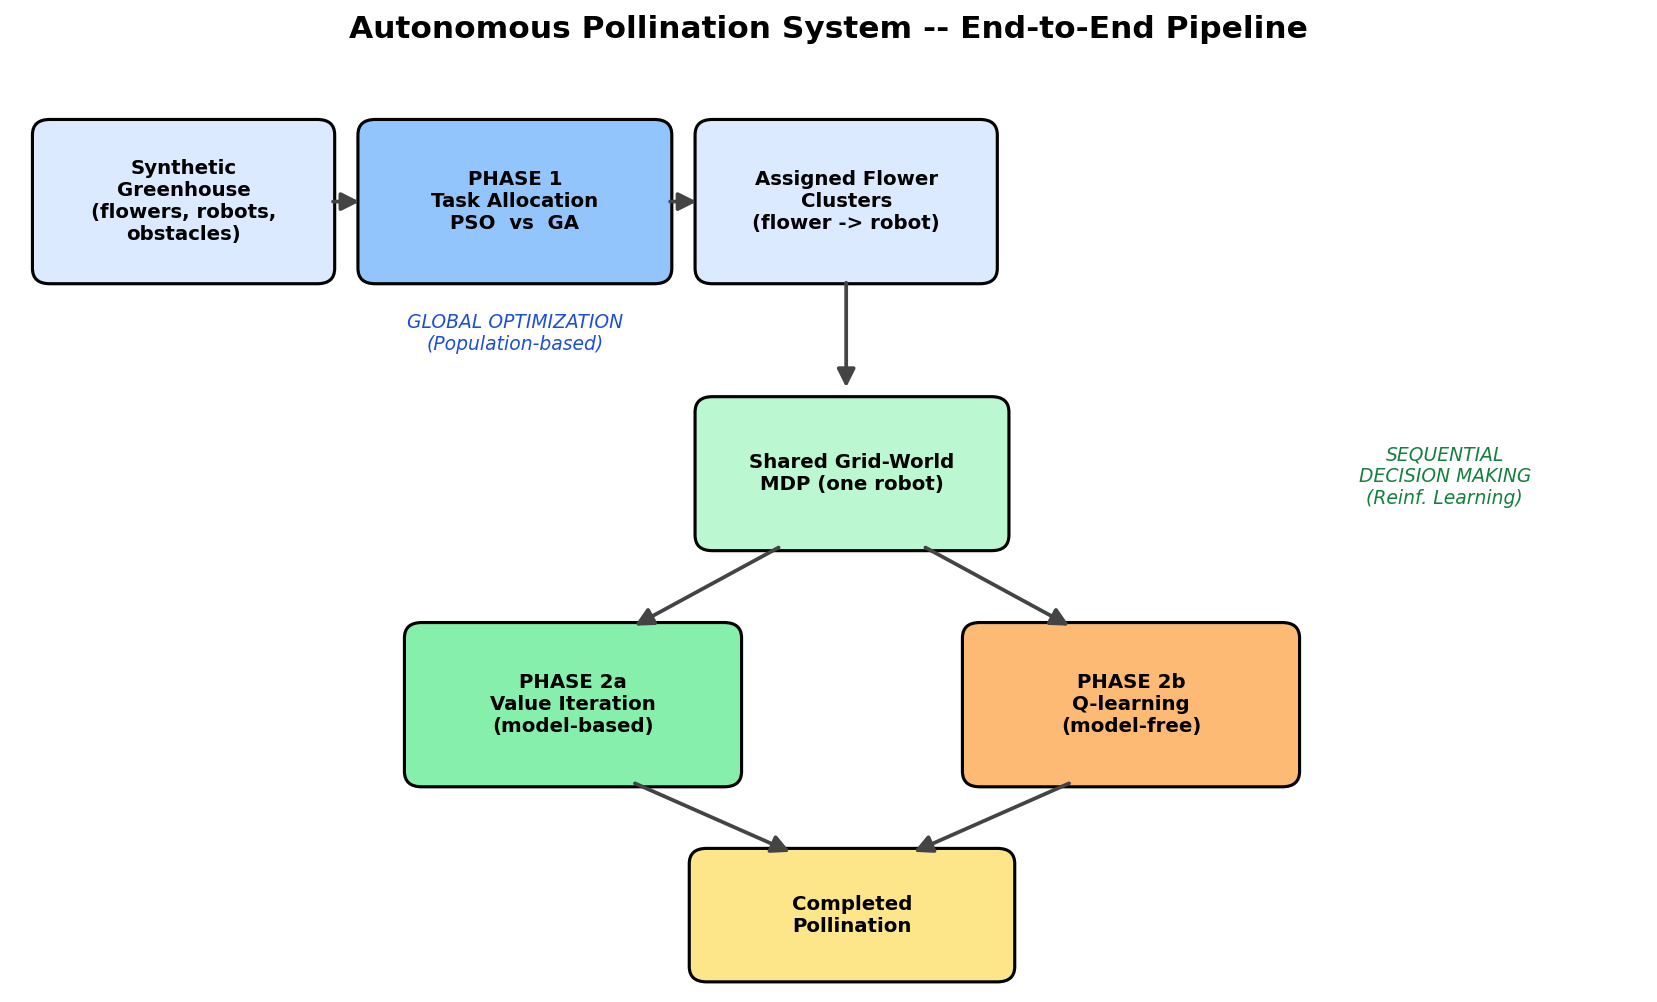
\includegraphics[width=\textwidth]{System/system_pipeline.png}
\caption{\textbf{End-to-end pipeline.} How the two AI paradigms connect,
read top-to-bottom.}
\end{figure}
\readhead
\begin{readlist}
  \item \textbf{Top row (blue boxes):} Phase~1. The synthetic greenhouse feeds
        the task allocator (``PSO vs GA''), which outputs flower clusters ---
        which robot owns which flowers.
  \item \textbf{Middle (green box):} those clusters define one \emph{shared
        grid-world MDP} for a single robot to navigate.
  \item \textbf{Two branches below:} Phase~2 solves that same grid two ways ---
        \emph{Value Iteration} (left, model-based) and \emph{Q-learning}
        (right, model-free).
  \item \textbf{Bottom (yellow box):} both branches re-join at ``Completed
        Pollination'' --- either method finishes the mission.
  \item \textbf{Italic side captions} name the paradigm of each half: global
        \emph{population-based} optimization on top, \emph{reinforcement
        learning} below.
\end{readlist}

\begin{figure}[H]
\centering
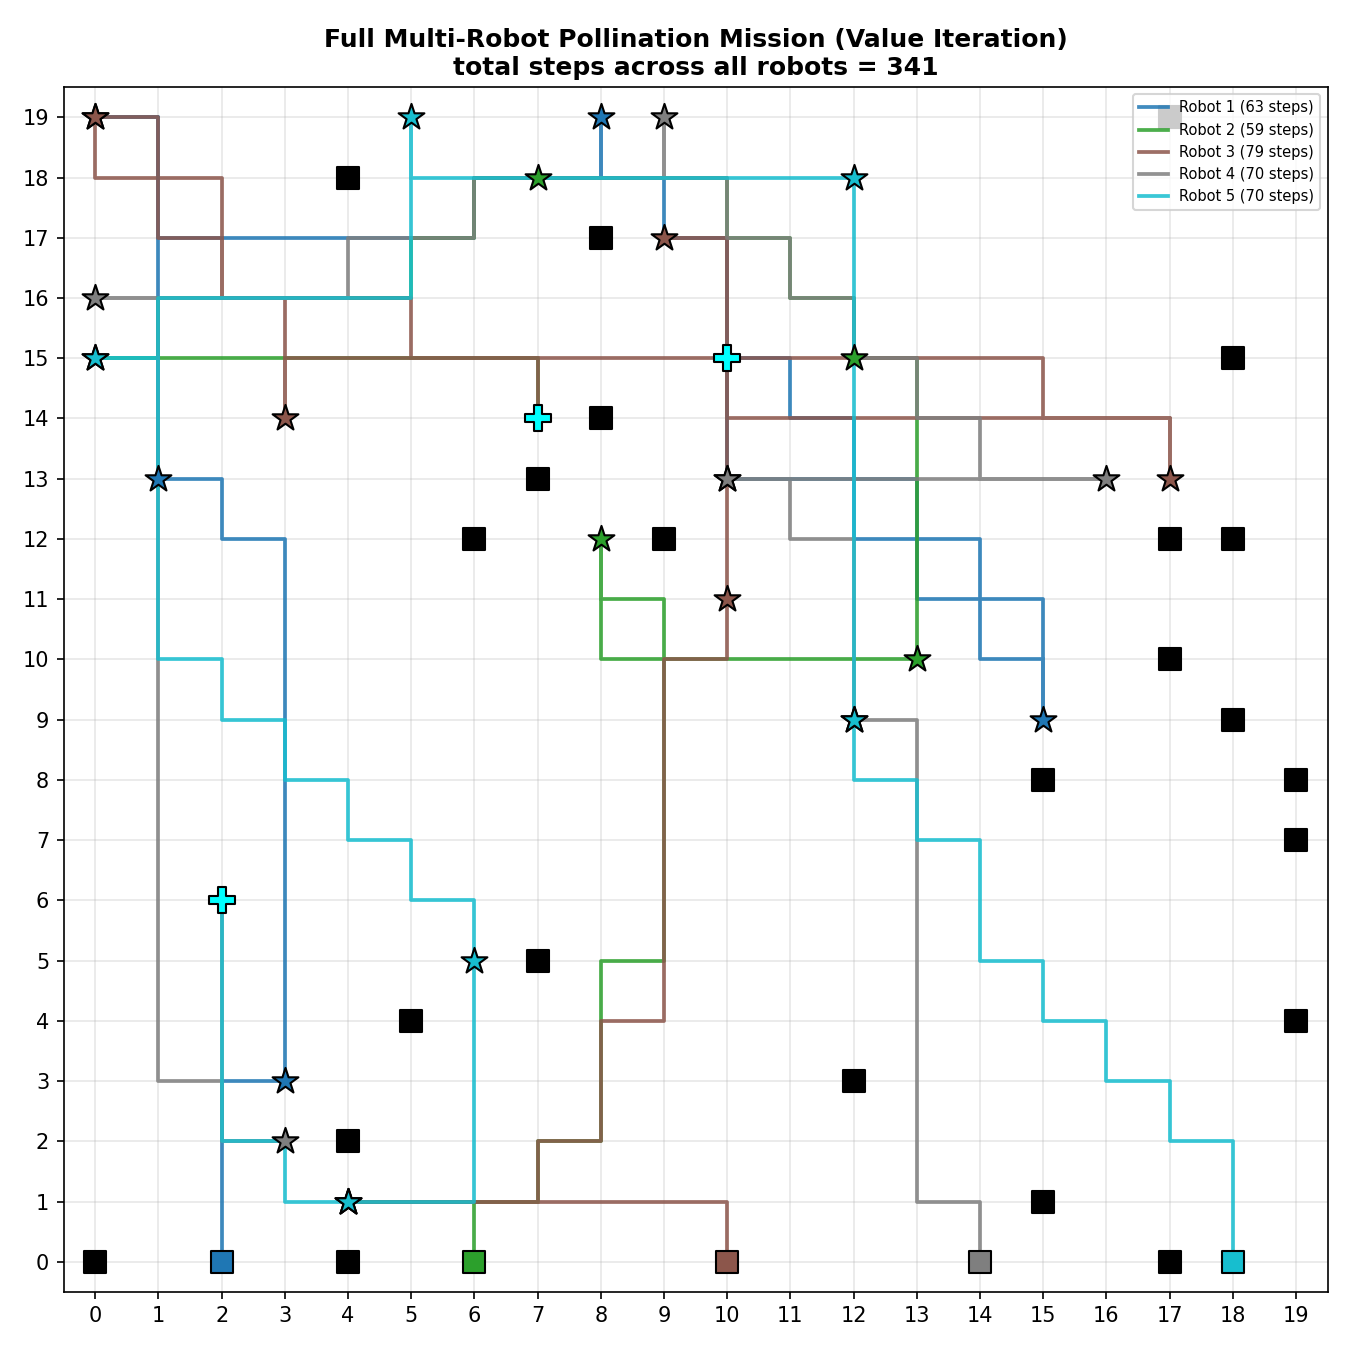
\includegraphics[width=0.72\textwidth]{System/all_robots_navigation.png}
\caption{\textbf{Full multi-robot mission.} All five robots navigating on one
grid.}
\end{figure}
\readhead
\begin{readlist}
  \item \textbf{Axes:} grid X and grid Y --- the greenhouse discretized into a
        $20\times20$ lattice of cells.
  \item \textbf{Each colour = one robot.} A robot's coloured line is its path;
        the coloured $\bigstar$ stars are the flowers assigned to that robot;
        the coloured square is where it starts.
  \item \textbf{Shared black squares} are obstacles; \textbf{cyan ``P''} are
        charging stations (common to all robots).
  \item \textbf{Title} reports the total steps summed over the whole fleet ---
        evidence the \emph{complete} system finishes, not just one robot.
\end{readlist}

% =====================================================================
\section{Phase 1 --- PSO Task Allocation}
% =====================================================================
PSO encodes an assignment as a continuous vector (one dimension per flower,
floored to a robot index) and minimizes the weighted multi-objective fitness
described in the notation key.

\begin{figure}[H]
\centering
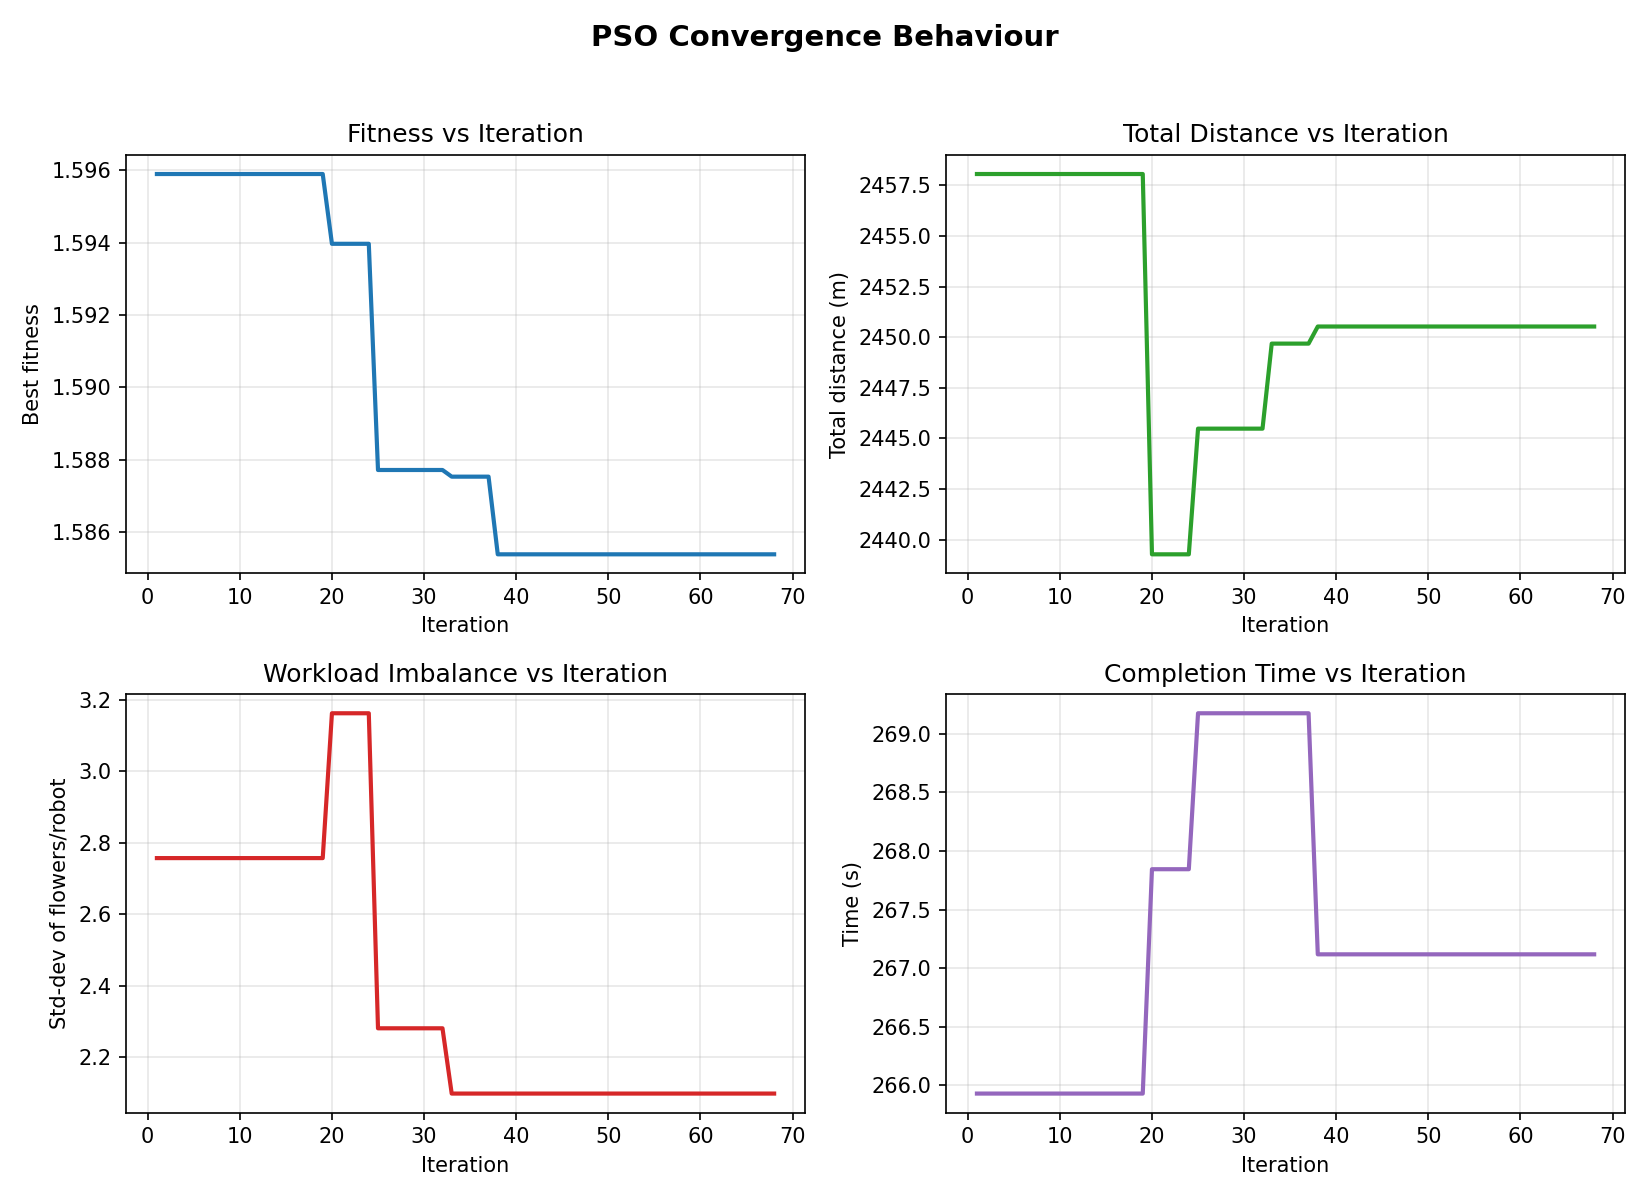
\includegraphics[width=0.9\textwidth]{PSO/pso_convergence.png}
\caption{\textbf{PSO convergence behaviour} --- four panels, all sharing the
x-axis \emph{iteration} (one full swarm update).}
\end{figure}
\readhead
\begin{readlist}
  \item Every panel plots the \emph{best-so-far} value, so a curve can never
        jump back up for fitness (the global best is remembered).
  \item \textbf{Top-left --- Fitness vs Iteration:} the overall cost. It falls
        and flattens: the swarm is improving, then converging. Lower = better.
  \item \textbf{Top-right --- Total Distance (m):} total flight distance of the
        current best allocation. It may wobble slightly because it is only
        \emph{one} of six competing terms.
  \item \textbf{Bottom-left --- Workload Imbalance ($\sigma$):} how unevenly
        flowers are split across robots. Falling means the split is getting
        fairer.
  \item \textbf{Bottom-right --- Completion Time (s):} the makespan (slowest
        robot's finish time). Also trends down.
  \item \textbf{Take-away:} fitness dropping while imbalance also drops shows
        PSO trading a little distance for a much fairer, cheaper plan overall.
\end{readlist}

\begin{figure}[H]
\centering
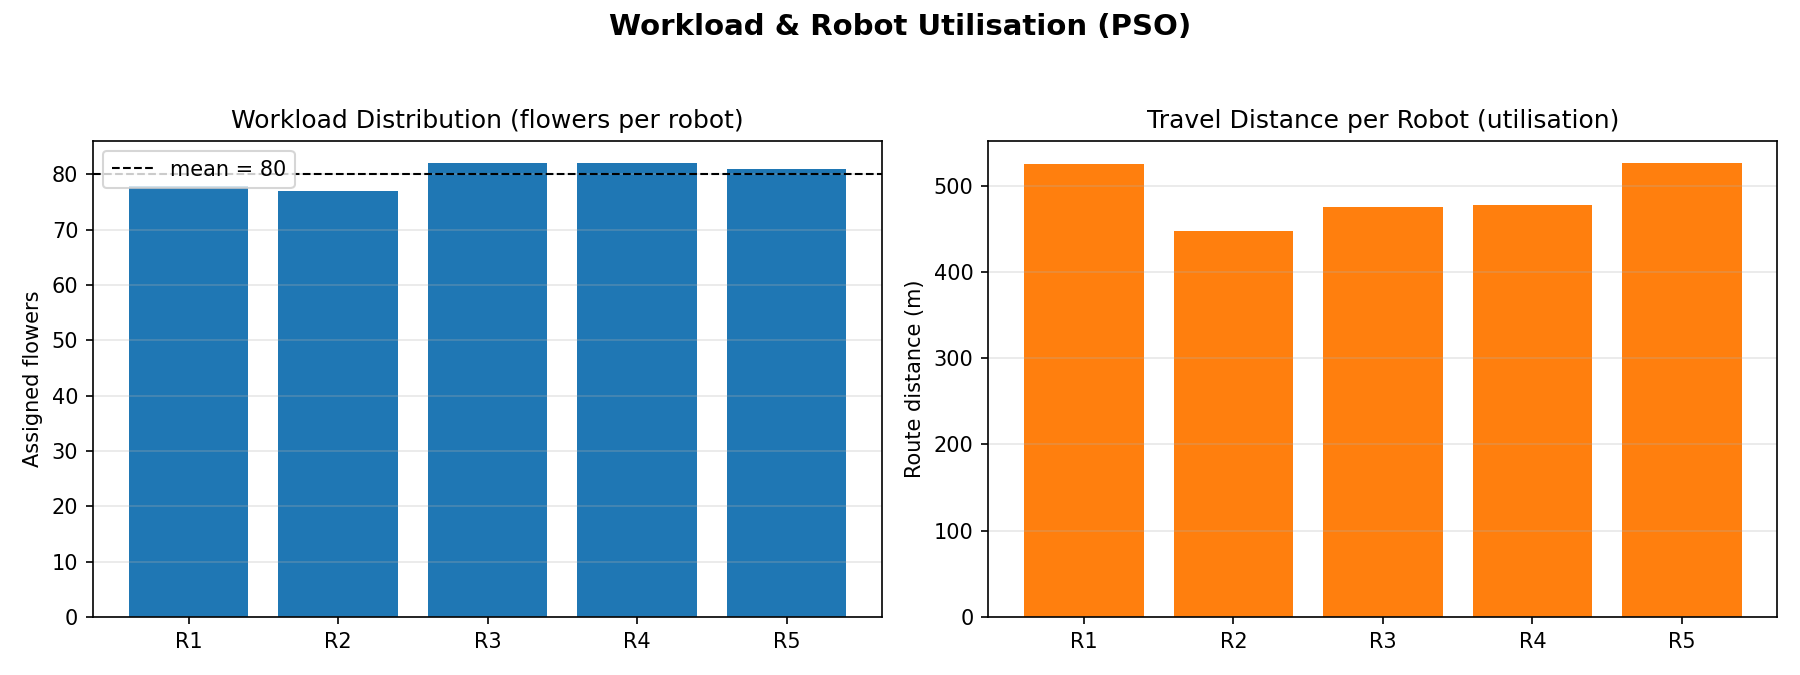
\includegraphics[width=0.9\textwidth]{PSO/pso_workload_utilisation.png}
\caption{\textbf{Workload and utilization} --- two bar charts. ``R1''$\dots$
``R5'' on the x-axis are the five robots.}
\end{figure}
\readhead
\begin{readlist}
  \item \textbf{Left --- Workload Distribution:} bar height = number of flowers
        assigned to each robot. The dashed horizontal line is the \emph{mean}
        ($\approx 80$). Bars hugging that line = a balanced workload.
  \item \textbf{Right --- Travel Distance per Robot:} bar height = how far that
        robot must fly. Similar heights mean no single robot is overworked.
  \item \textbf{Take-away:} PSO gives every robot work and keeps both the flower
        counts and the flight distances even.
\end{readlist}

\begin{figure}[H]
\centering
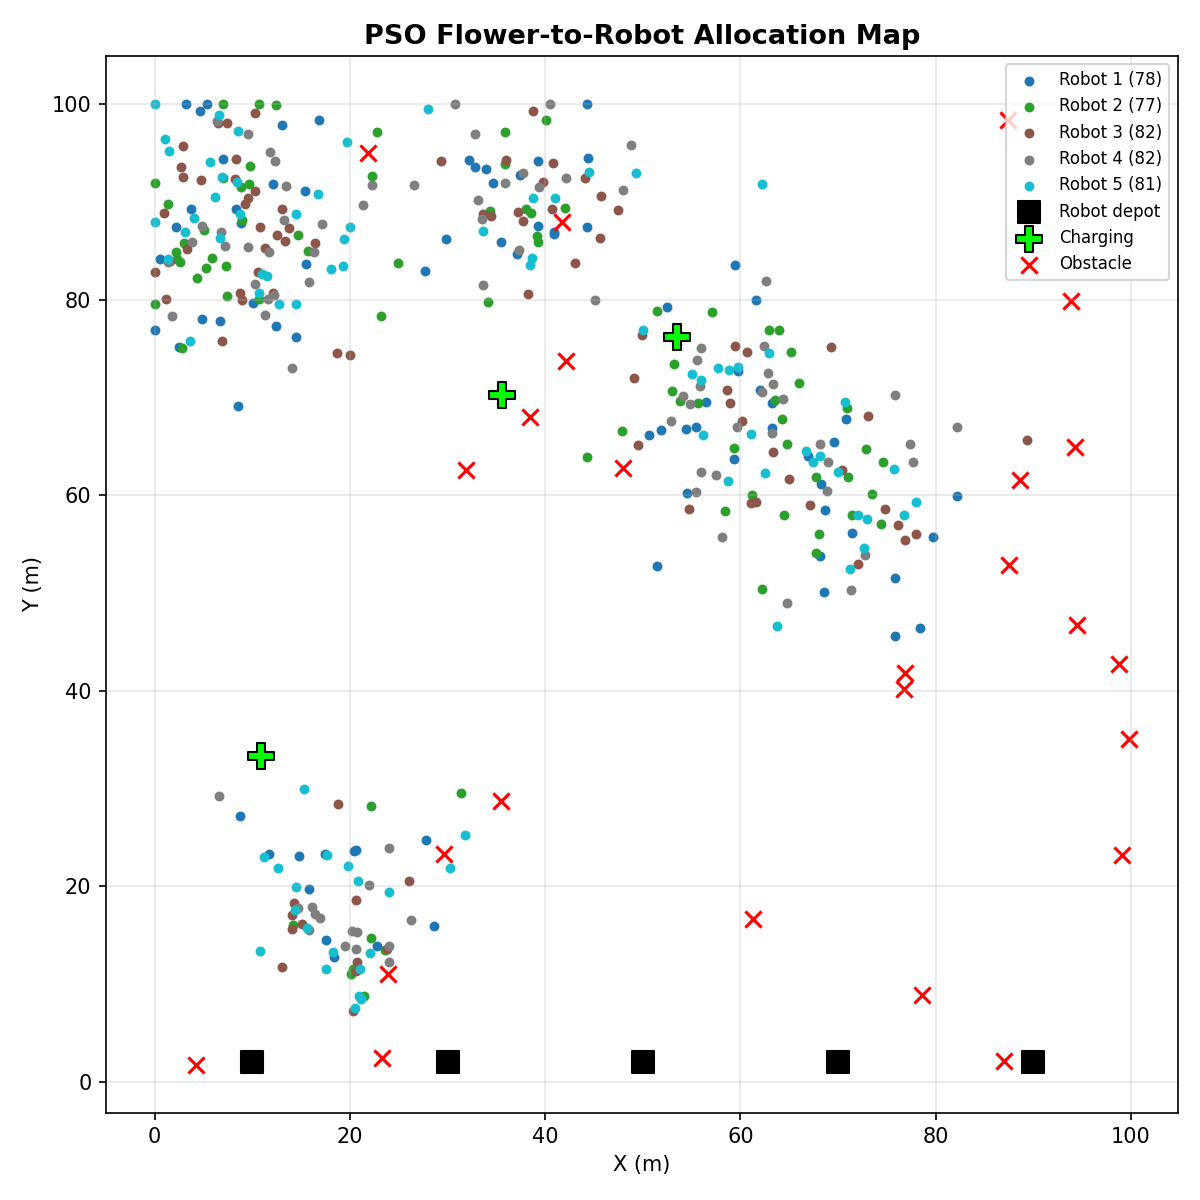
\includegraphics[width=0.7\textwidth]{PSO/pso_allocation_map.png}
\caption{\textbf{PSO allocation map} --- the greenhouse coloured by which robot
owns each flower.}
\end{figure}
\readhead
\begin{readlist}
  \item \textbf{Axes:} X and Y in metres --- real positions inside the
        $100\times100$\,m greenhouse.
  \item \textbf{Small dots:} flowers, coloured by the robot assigned to them;
        the legend gives each robot's flower count.
  \item \textbf{Black squares:} robot depots (start points). \textbf{Lime
        ``P'':} charging stations. \textbf{Red $\times$:} obstacles.
  \item \textbf{Take-away:} because PSO searches a huge continuous space, its
        colours stay intermixed and it is only modestly better than random ---
        which motivates the Genetic Algorithm next.
\end{readlist}

\begin{figure}[H]
\centering
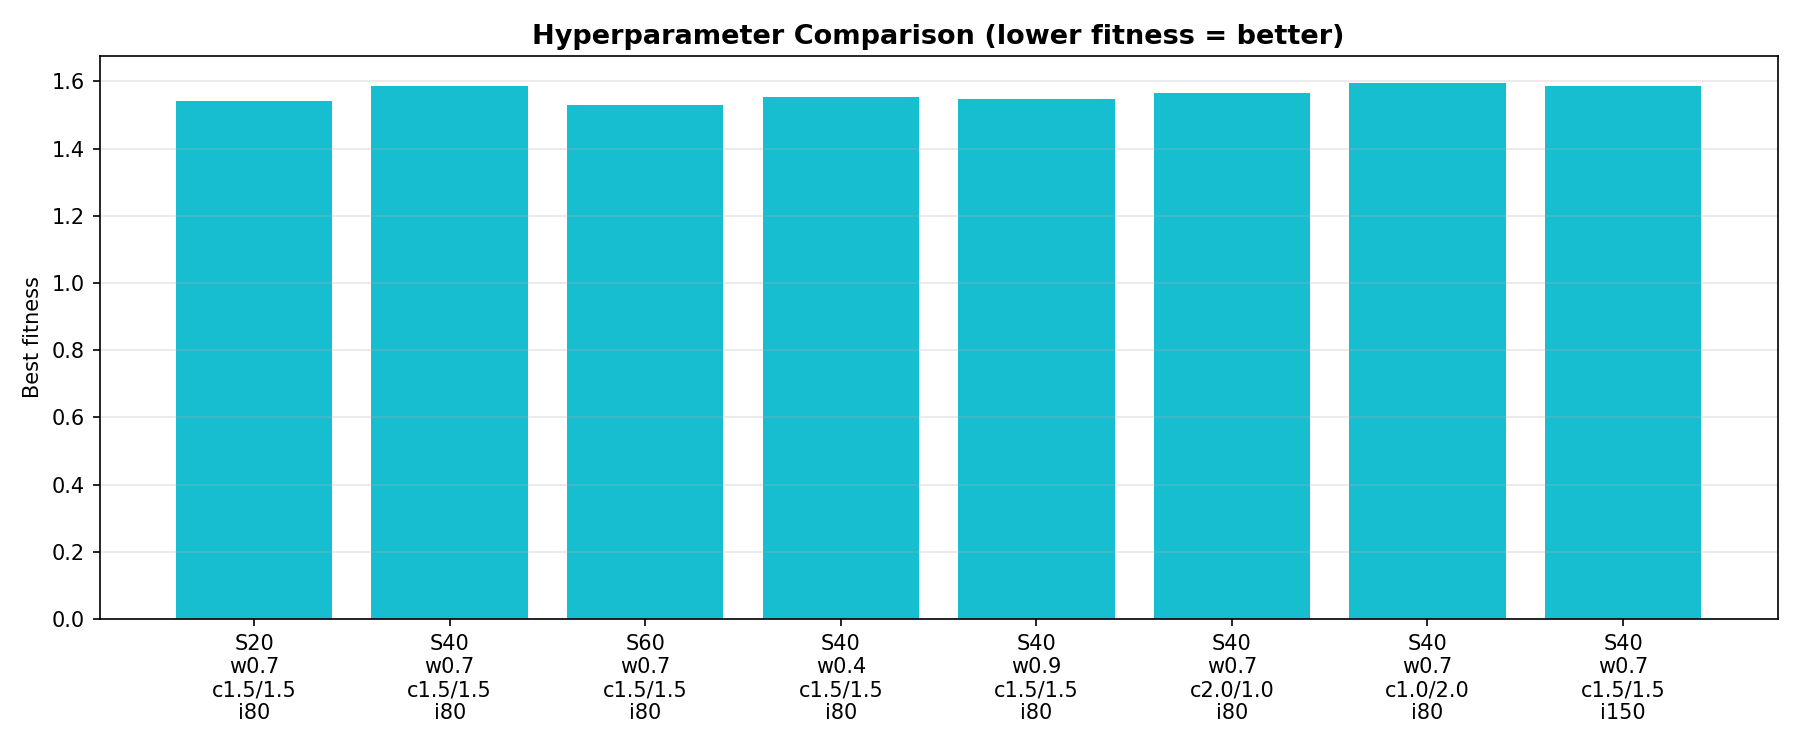
\includegraphics[width=\textwidth]{PSO/pso_hyperparameter_comparison.png}
\caption{\textbf{PSO hyperparameter study} --- one bar per configuration.}
\end{figure}
\readhead
\begin{readlist}
  \item \textbf{Each bar = one PSO setting.} The x-axis label encodes it:
        \texttt{S}=swarm size, \texttt{w}=inertia, \texttt{c}=$c_1/c_2$
        (cognitive/social), \texttt{i}=iterations.
  \item \textbf{Bar height = best fitness reached} with that setting. Lower is
        better.
  \item \textbf{Take-away:} the flat-ish bars show PSO is fairly robust to its
        settings; the lowest bar justifies the default configuration used
        everywhere else.
\end{readlist}

% =====================================================================
\section{Phase 1 --- GA Task Allocation (vs.\ PSO)}
% =====================================================================
A Genetic Algorithm solves the \emph{same} allocation problem with a
\emph{discrete} encoding: a chromosome is 400 genes (one robot index per
flower). It evolves a population using tournament selection, uniform crossover,
random-reset mutation and elitism, seeded with a distance-greedy assignment.

\begin{figure}[H]
\centering
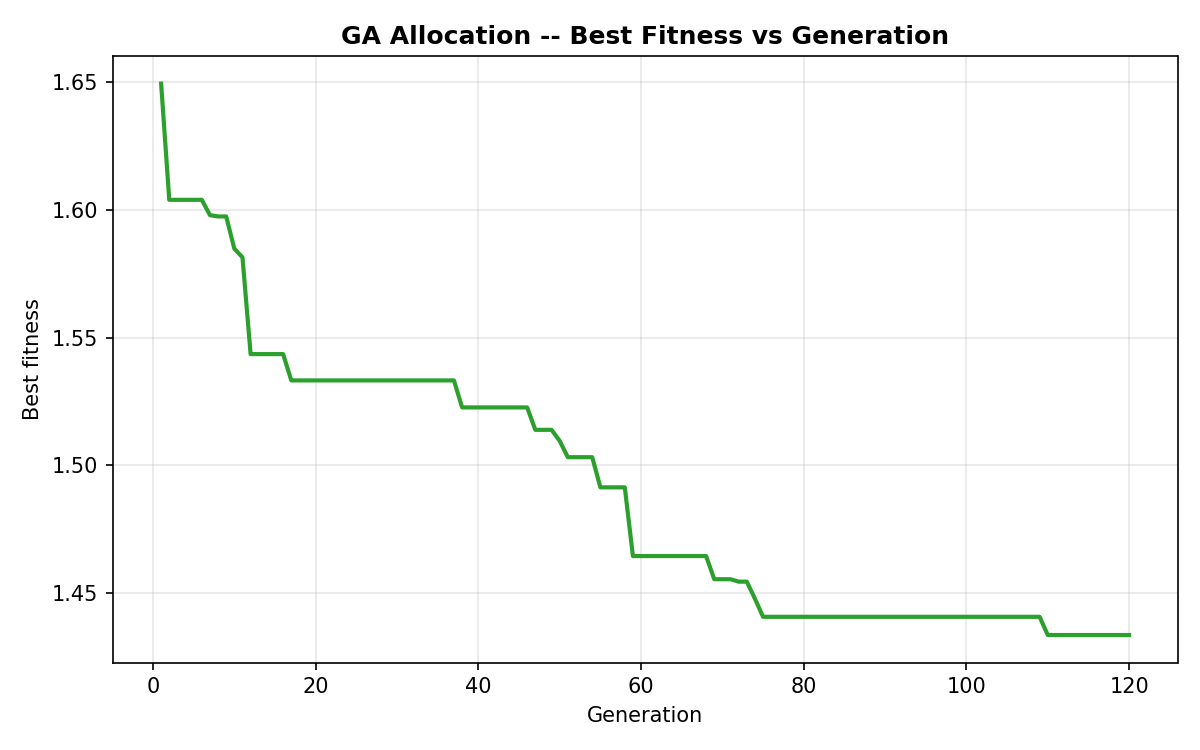
\includegraphics[width=0.75\textwidth]{GA/ga_alloc_convergence.png}
\caption{\textbf{GA allocation convergence} --- a single curve.}
\end{figure}
\readhead
\begin{readlist}
  \item \textbf{x-axis:} generation (one full cycle of select $\rightarrow$
        crossover $\rightarrow$ mutate). \textbf{y-axis:} best fitness so far.
  \item The curve only ever goes \emph{down} because \emph{elitism} always
        keeps the best chromosome --- the population can never get worse.
  \item \textbf{Numbers to note:} it falls from $\approx1.6$ to $\approx1.43$,
        landing \emph{below} PSO's $\approx1.59$ --- the GA finds a better plan.
\end{readlist}

\begin{figure}[H]
\centering
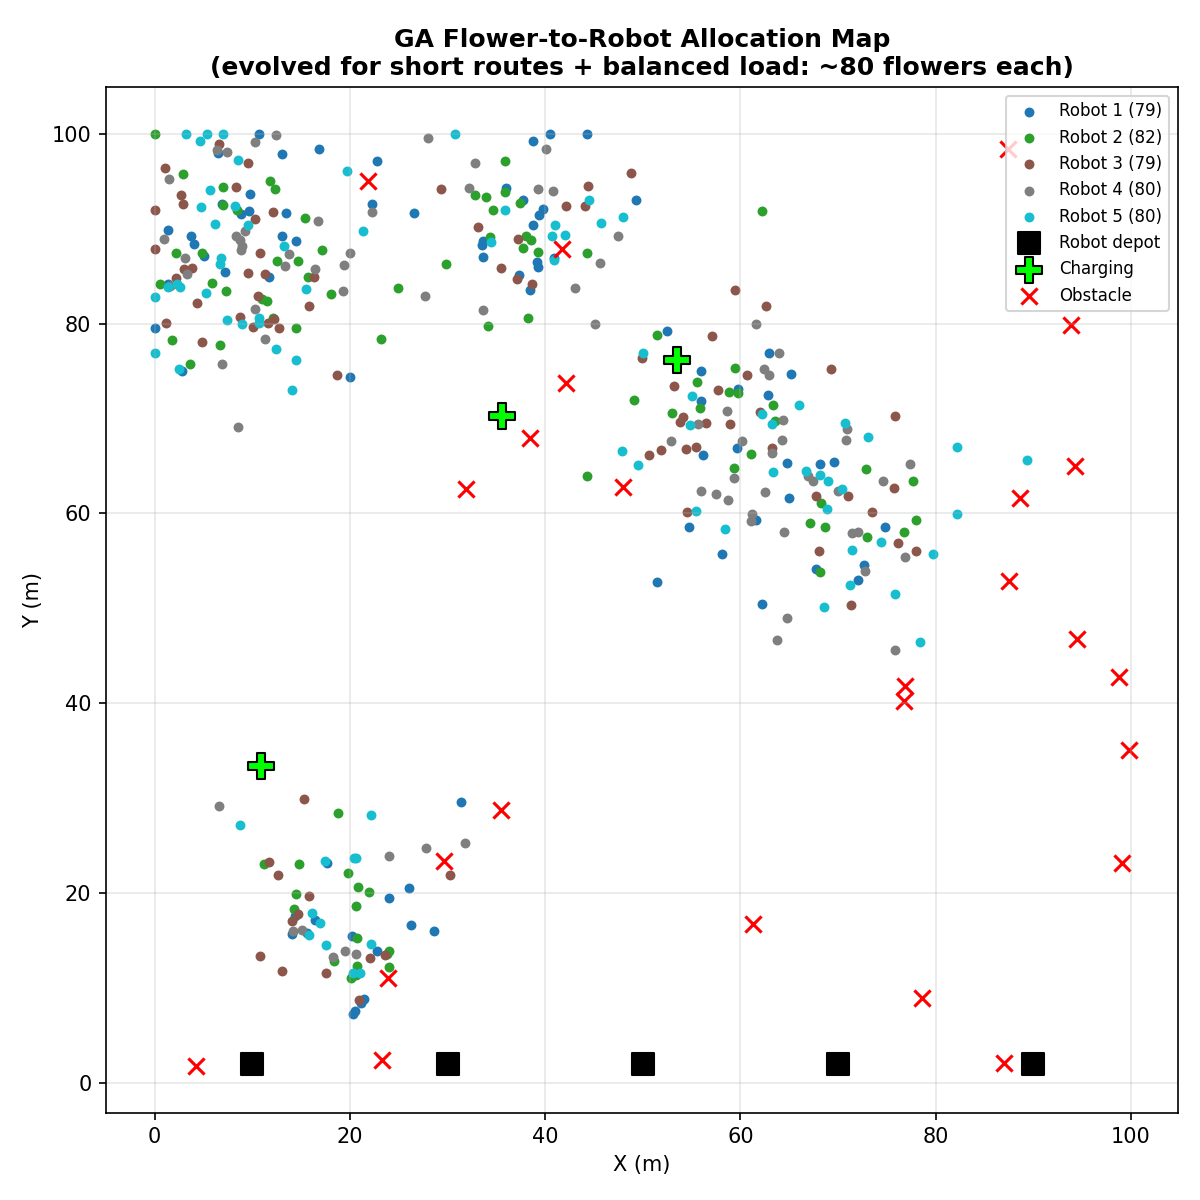
\includegraphics[width=0.7\textwidth]{GA/ga_alloc_map.png}
\caption{\textbf{GA allocation map} --- same greenhouse, coloured by the GA's
assignment (same markers as the PSO map).}
\end{figure}
\readhead
\begin{readlist}
  \item Read the markers exactly as the PSO map (dots = flowers by robot, black
        squares = depots, lime ``P'' = charging, red $\times$ = obstacles).
  \item \textbf{Legend counts:} every robot gets $79$--$82$ of the $400$
        flowers --- an almost perfectly even split.
  \item \textbf{Important honesty note:} the colours look just as intermixed as
        PSO's. That is expected --- the $400$ flowers sit in a few dense
        clusters that \emph{must be shared} to keep loads balanced. The GA's win
        is \emph{quantitative} (shorter total routes, tighter balance, lower
        fitness), \emph{not} a visually neater map.
\end{readlist}

\begin{figure}[H]
\centering
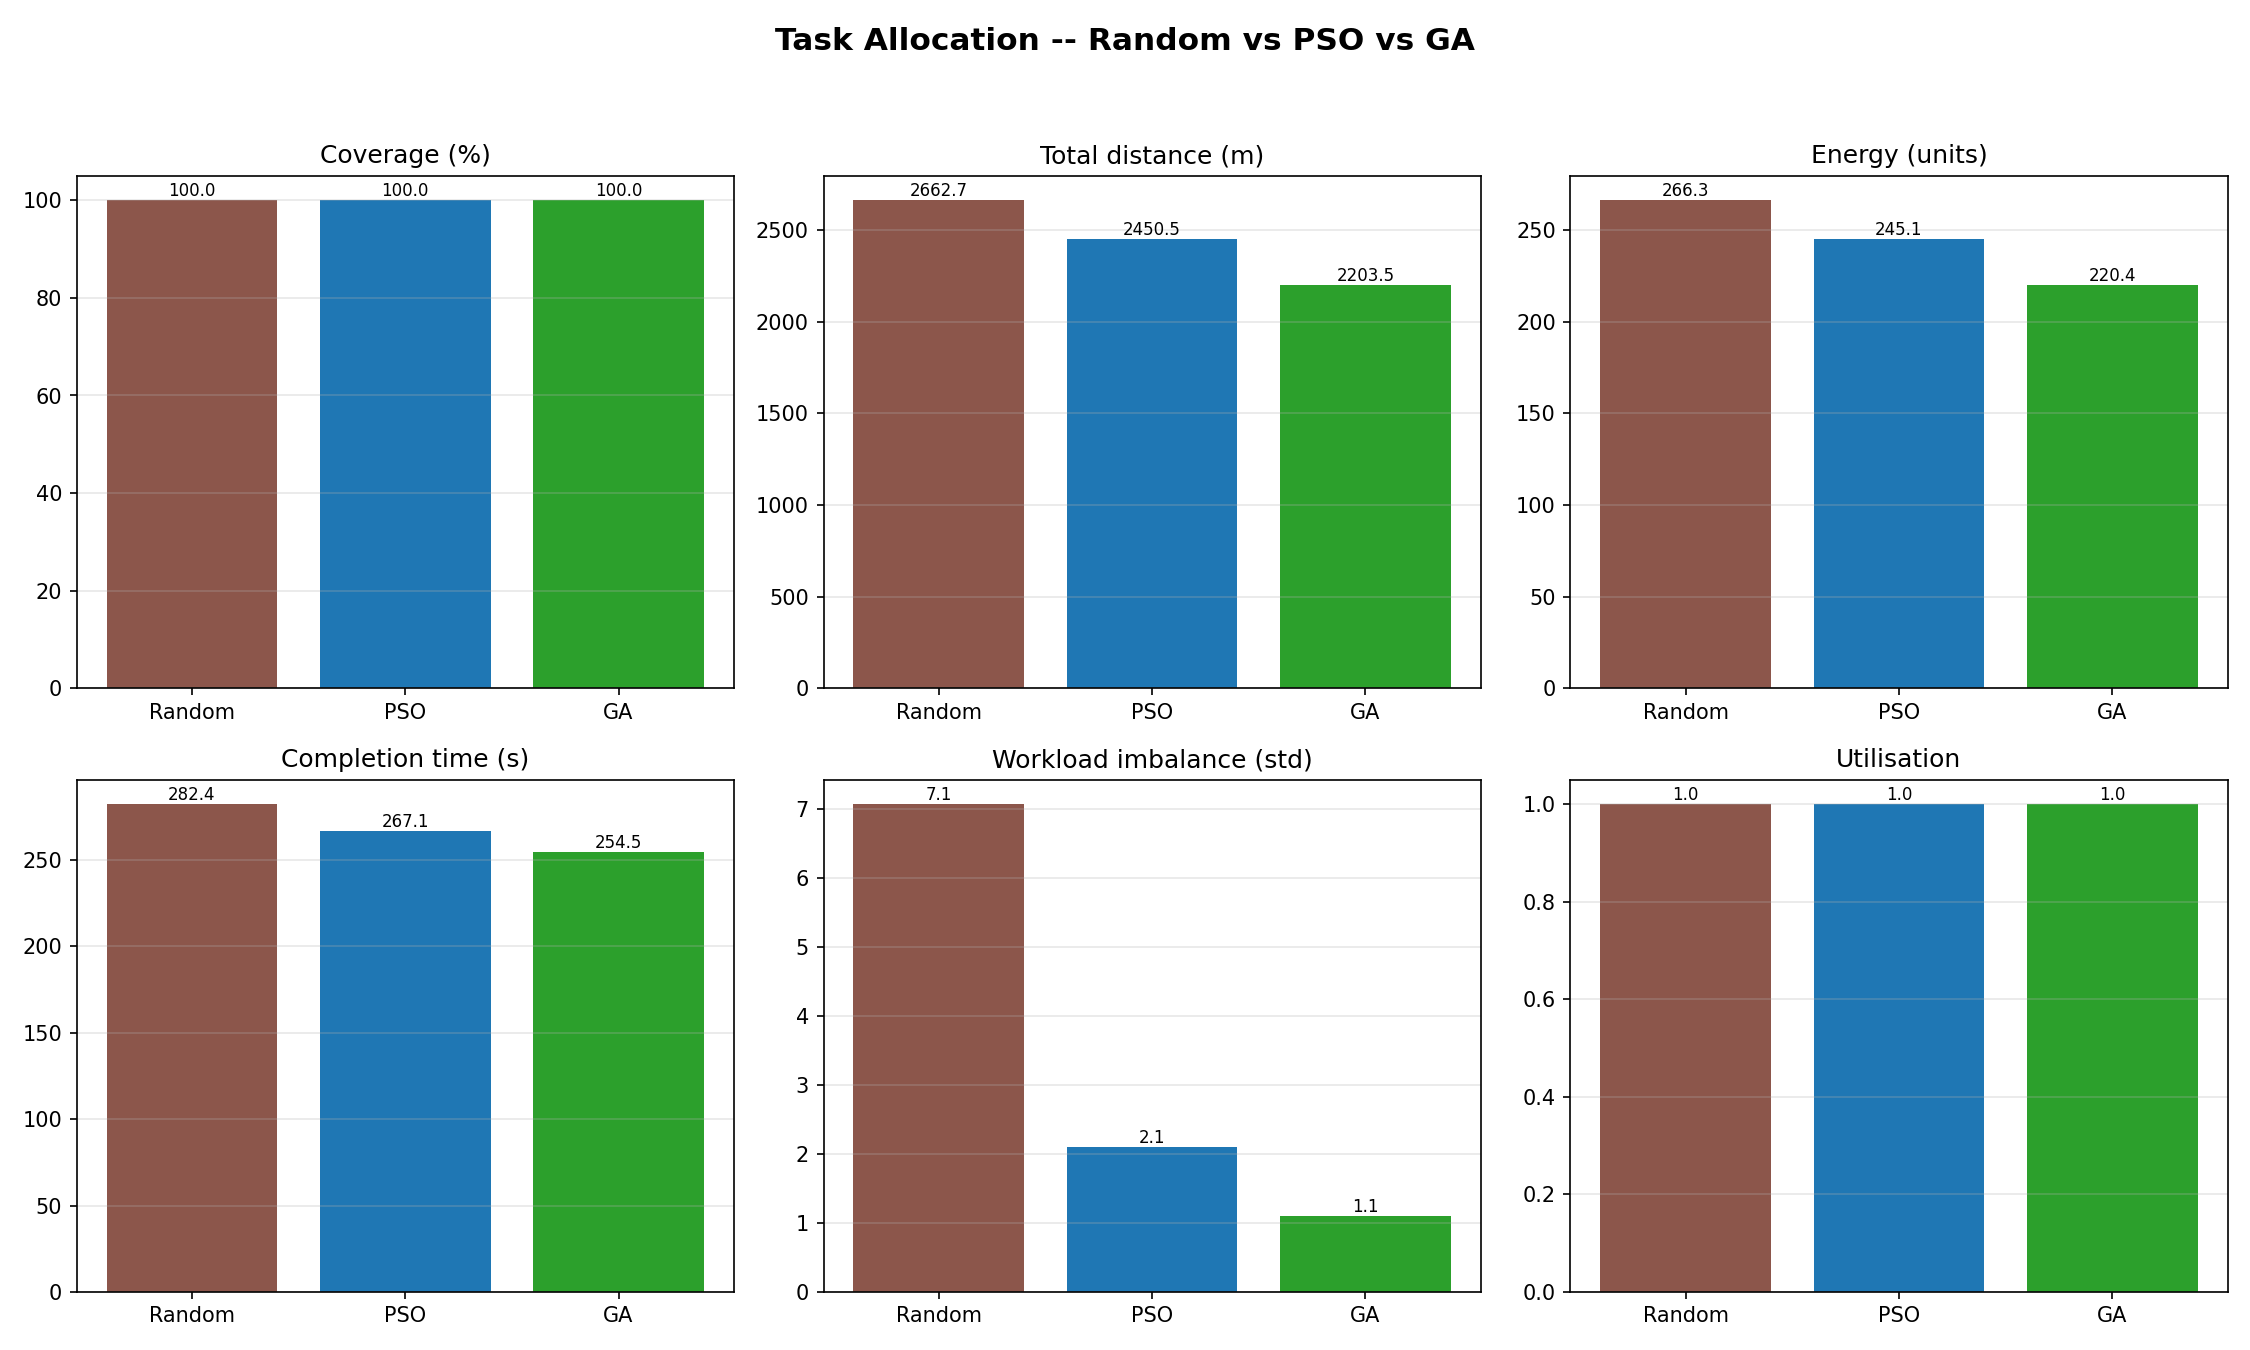
\includegraphics[width=\textwidth]{Comparison/pso_vs_ga_allocation.png}
\caption{\textbf{Random vs.\ PSO vs.\ GA allocation} --- six panels, one per
objective. In each panel the three bars are Random, PSO and GA.}
\end{figure}
\readhead
\begin{readlist}
  \item \textbf{Bar labels} print the exact value on top of every bar.
  \item \textbf{Coverage (\%)} and \textbf{Utilisation:} higher is better
        (all three reach $100\%$ here).
  \item \textbf{Total distance, Energy, Completion time, Workload $\sigma$:}
        \emph{lower} is better. The GA (rightmost bar) is lowest in every one
        of these four panels.
  \item \textbf{Take-away --- the central Phase~1 result:} on the combined
        objective the GA is the strongest allocator, beating PSO which beats
        Random.
\end{readlist}

\begin{figure}[H]
\centering
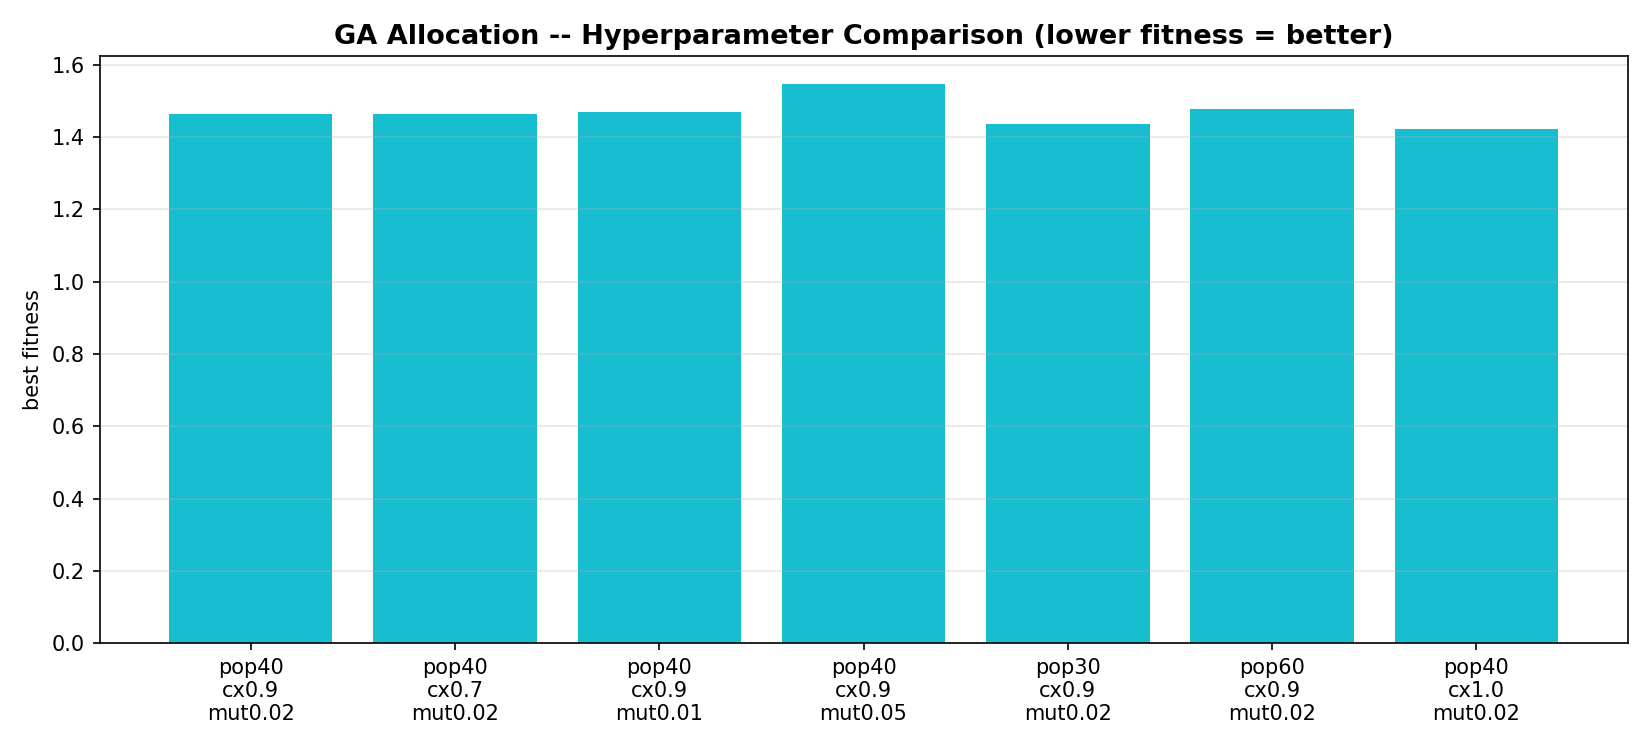
\includegraphics[width=\textwidth]{GA/ga_alloc_hyperparameter_comparison.png}
\caption{\textbf{GA allocation hyperparameter study} --- one bar per
configuration.}
\end{figure}
\readhead
\begin{readlist}
  \item \textbf{x-axis label} encodes the setting: \texttt{pop}=population size,
        \texttt{cx}=crossover rate, \texttt{mut}=mutation rate.
  \item \textbf{Bar height = best fitness} (lower is better).
  \item \textbf{Take-away:} the tall (bad) bar at a high mutation rate
        ($0.05$) shows too much random change destroys good chromosomes ---
        confirming that \emph{small mutation + strong crossover} is the right
        balance.
\end{readlist}

% =====================================================================
\section{Phase 2 --- Value Iteration (model-based)}
% =====================================================================
The environment is fully known. Value Iteration applies the Bellman optimality
update
$U(s)=\max_a\sum_{s'}T(s,a,s')\,[\,R(s,a,s')+\gamma\,U(s')\,]$
on a stochastic grid-world MDP until convergence, then extracts the greedy
policy. The transition reward $R$ is $-0.1$ for a normal step and $-5$ for a
move blocked by a wall, so VI feels the \emph{same} collision penalty as
Q-learning.

\begin{figure}[H]
\centering
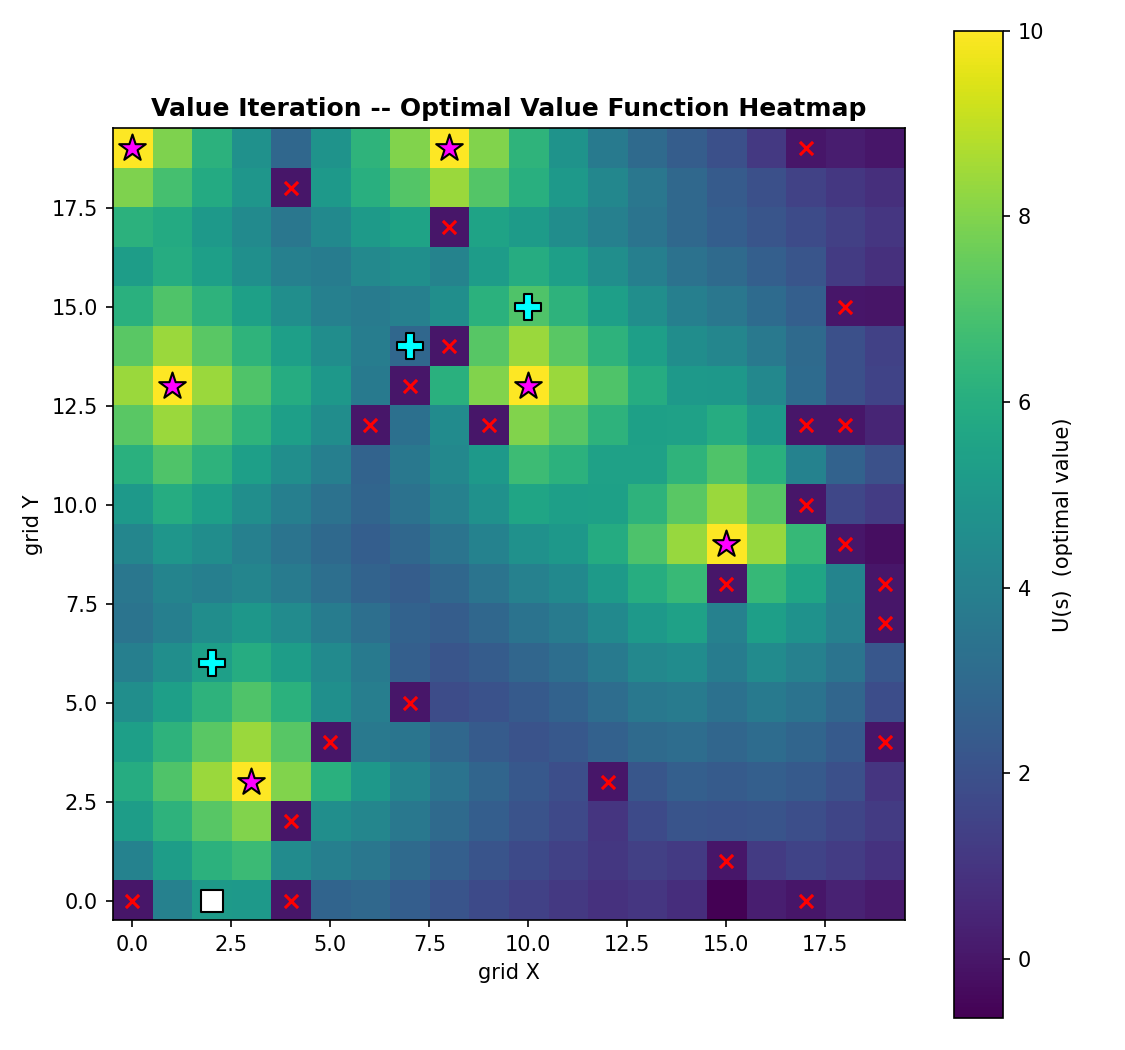
\includegraphics[width=0.62\textwidth]{ValueIteration/vi_value_heatmap.png}
\caption{\textbf{Optimal value function $U(s)$} --- a heat map over the grid.}
\end{figure}
\readhead
\begin{readlist}
  \item \textbf{Colour = value $U(s)$} of each cell (see the colourbar on the
        right): bright yellow = high value (good place to be), dark purple =
        low value.
  \item Value is \textbf{highest at the flowers} and \emph{fades smoothly} with
        distance --- like a hill with flowers at the peaks.
  \item \textbf{Markers:} $\bigstar$ magenta = flower, red $\times$ = obstacle,
        cyan ``P'' = charging, white square = start.
  \item \textbf{Take-away:} a robot only has to walk ``uphill'' on this surface
        to reach a flower --- exactly what a correct value function should look
        like.
\end{readlist}

\begin{figure}[H]
\centering
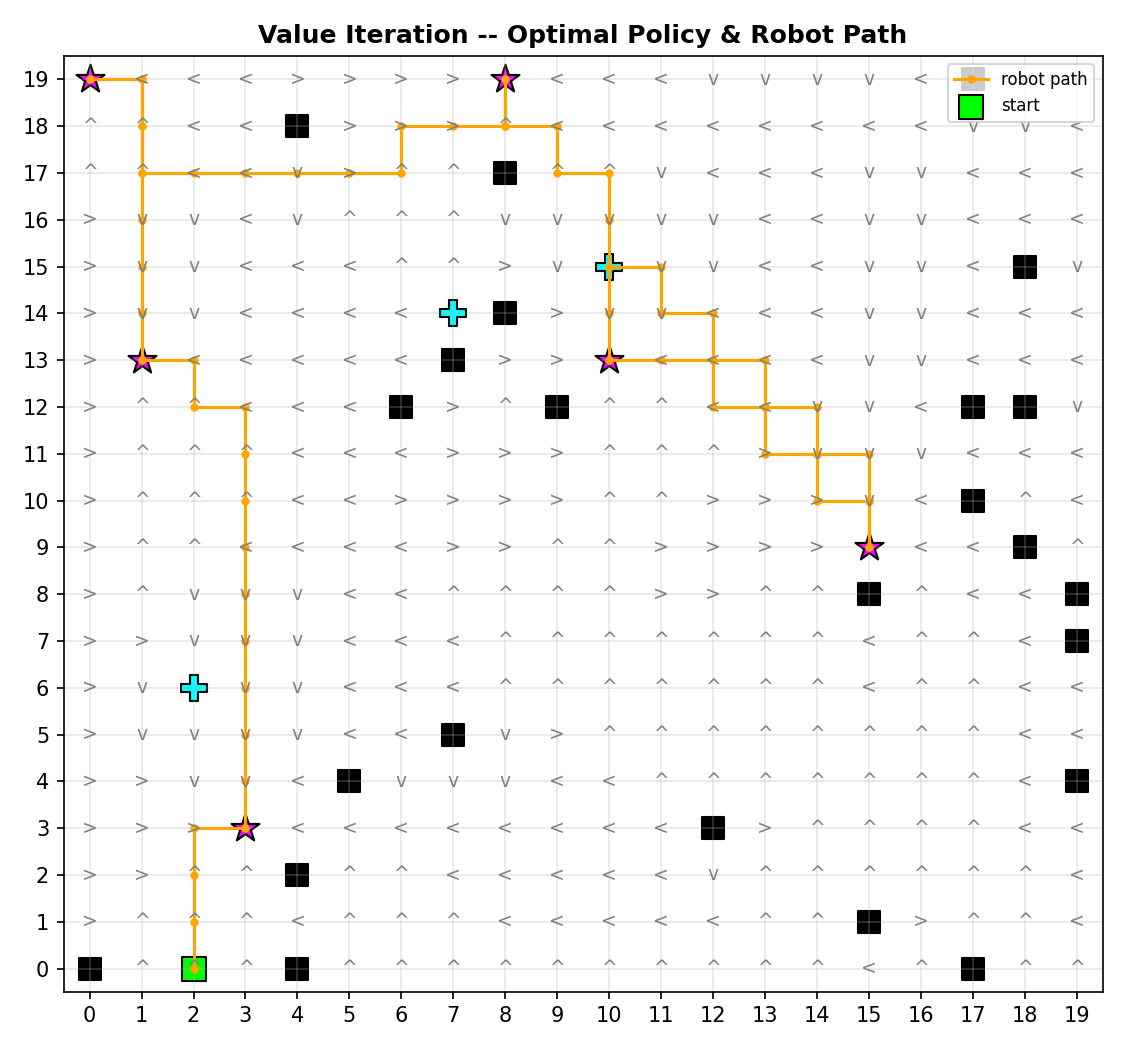
\includegraphics[width=0.62\textwidth]{ValueIteration/vi_policy.png}
\caption{\textbf{Optimal policy and executed path.}}
\end{figure}
\readhead
\begin{readlist}
  \item \textbf{Grey arrows:} the policy --- the best action in every cell
        ($\uparrow\downarrow\leftarrow\rightarrow$). Follow the arrows from any
        cell and you reach a flower optimally.
  \item \textbf{Orange line with dots:} the robot's actual executed mission ---
        visiting all flowers, then returning to charge.
  \item \textbf{Markers:} lime square = start, $\bigstar$ = flowers, cyan ``P''
        = charging, black squares = obstacles.
  \item \textbf{Take-away:} the orange path faithfully follows the grey arrows
        into the high-value regions --- policy and value agree.
\end{readlist}

\begin{figure}[H]
\centering
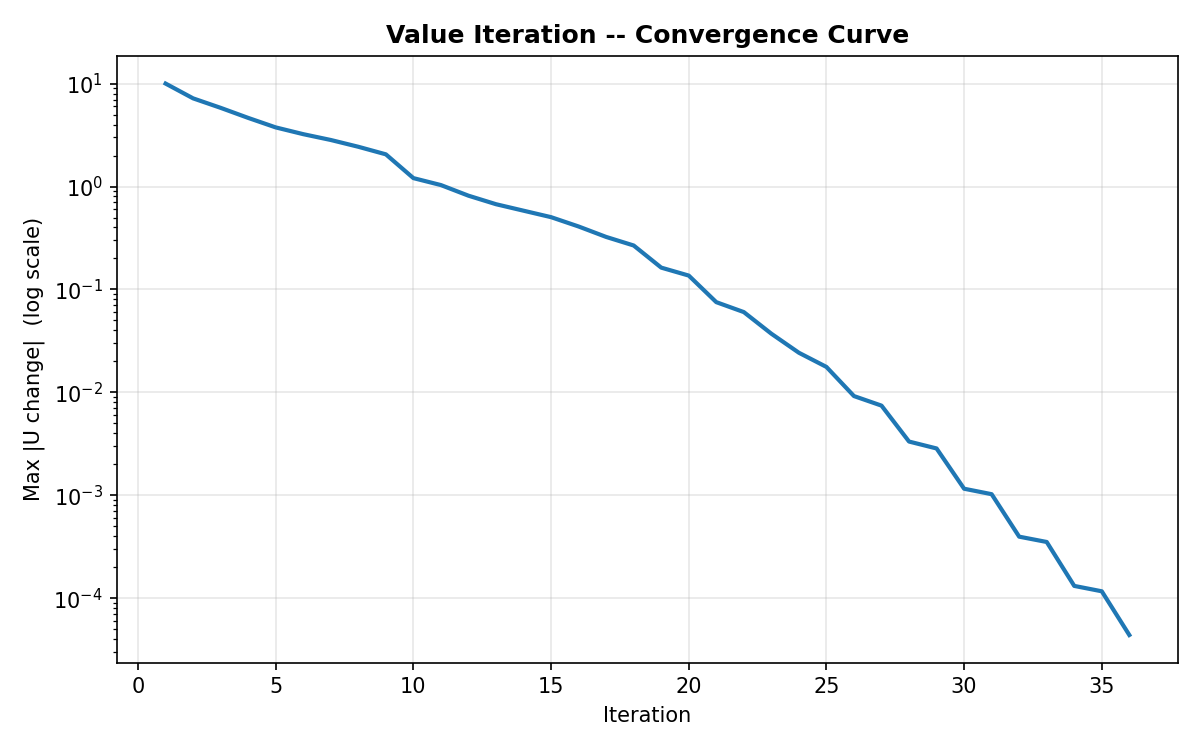
\includegraphics[width=0.68\textwidth]{ValueIteration/vi_convergence.png}
\caption{\textbf{Value Iteration convergence} --- note the \emph{logarithmic}
y-axis.}
\end{figure}
\readhead
\begin{readlist}
  \item \textbf{x-axis:} iteration (one Bellman sweep over all cells).
  \item \textbf{y-axis (log scale):} the biggest change in any cell's value that
        sweep, $\max_s|U_{k+1}(s)-U_k(s)|$. As it shrinks, the values are
        settling.
  \item A \textbf{straight line on a log axis} means the error shrinks by a
        constant factor each step --- \emph{geometric} (fast, guaranteed)
        convergence.
  \item \textbf{Take-away:} it crosses the stop threshold $\theta$ in about
        $36$ iterations.
\end{readlist}

\begin{figure}[H]
\centering
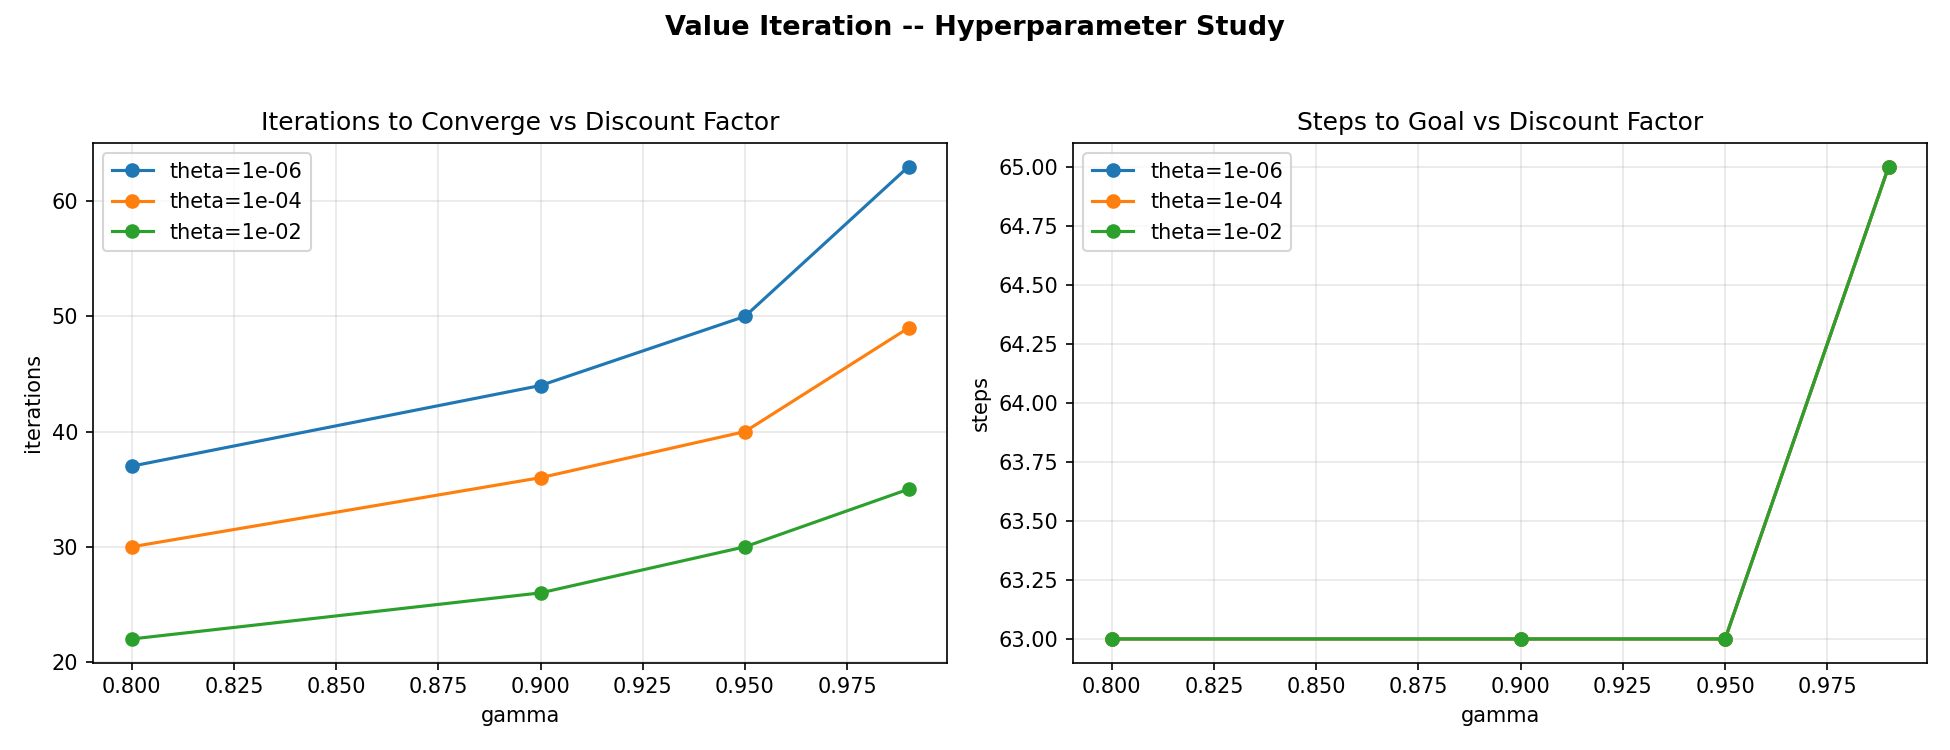
\includegraphics[width=\textwidth]{ValueIteration/vi_hyperparameters.png}
\caption{\textbf{Value Iteration hyperparameter study} --- two panels versus
the discount factor $\gamma$ (x-axis), one line per threshold $\theta$.}
\end{figure}
\readhead
\begin{readlist}
  \item \textbf{Left --- Iterations to Converge vs $\gamma$:} a bigger $\gamma$
        (more far-sighted) spreads value further, so it needs \emph{more}
        sweeps; a smaller $\theta$ (stricter stop) also needs more. Each line
        is one $\theta$ value.
  \item \textbf{Right --- Steps to Goal vs $\gamma$:} the length of the planned
        path. It stays essentially \emph{flat} at $\approx63$ steps.
  \item \textbf{Take-away:} these settings change only the \emph{compute cost}
        (left), not the \emph{quality} of the final path (right) --- the
        optimal route is the same either way.
\end{readlist}

\begin{figure}[H]
\centering
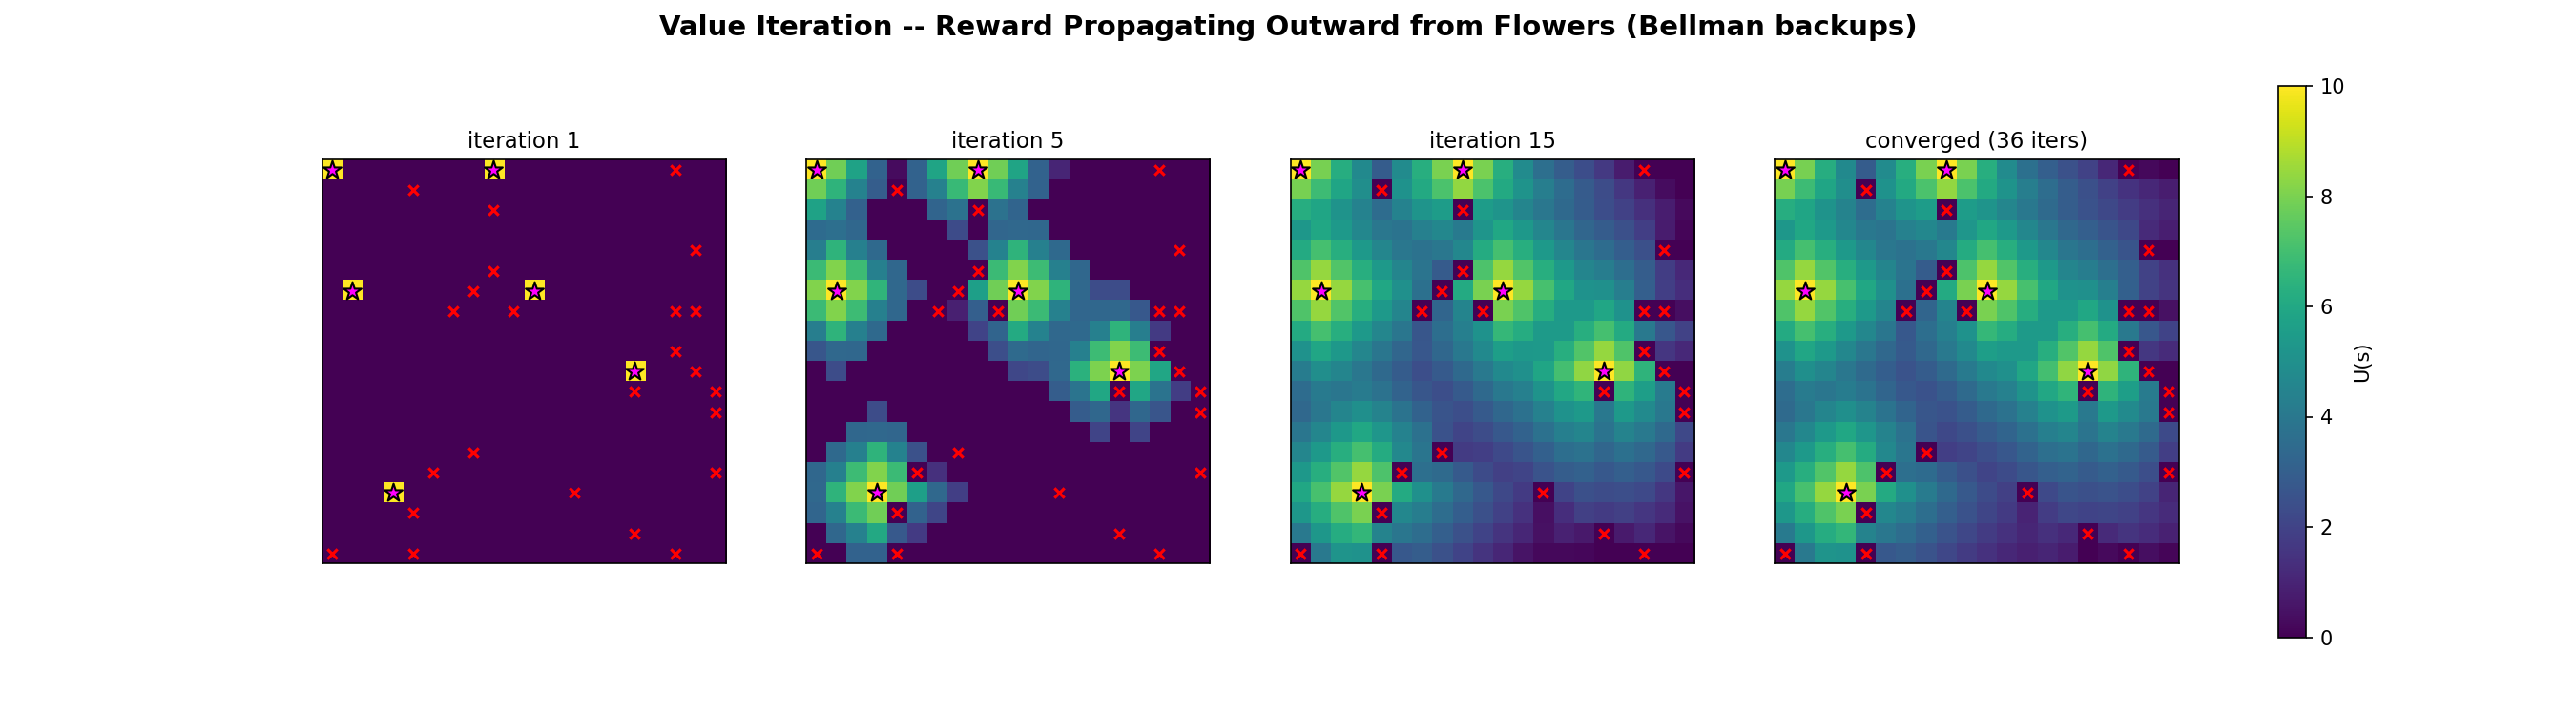
\includegraphics[width=\textwidth]{ValueIteration/vi_value_propagation.png}
\caption{\textbf{Value propagation} --- four heat-map snapshots, left to right,
after 1, 5, 15 and (converged) iterations.}
\end{figure}
\readhead
\begin{readlist}
  \item All four use the same colour scale (colourbar on the right,
        $U(s)$ from $0$ to $10$); $\bigstar$ = flower, red $\times$ = obstacle.
  \item \textbf{Panel 1 (iteration 1):} only cells \emph{touching} a flower are
        bright --- value has spread one ring.
  \item \textbf{Panels 2--3 (iterations 5, 15):} the bright region grows
        outward, ring by ring.
  \item \textbf{Panel 4 (converged):} the whole reachable grid has a sensible
        value pointing back to the flowers.
  \item \textbf{Take-away:} this literally shows the Bellman update ``backing
        up'' reward one step per sweep --- an intuitive picture of how Value
        Iteration works.
\end{readlist}

% =====================================================================
\section{Phase 2 --- Q-learning (model-free)}
% =====================================================================
The environment is treated as unknown. The agent learns by trial and error
with an $\varepsilon$-greedy policy and the update
$Q(s,a)\leftarrow Q(s,a)+\alpha\,[\,r+\gamma\max_{a'}Q(s',a')-Q(s,a)\,]$.
The state is augmented with a bitmask of already-pollinated flowers so the
memoryless agent can complete the multi-flower mission.

\begin{figure}[H]
\centering
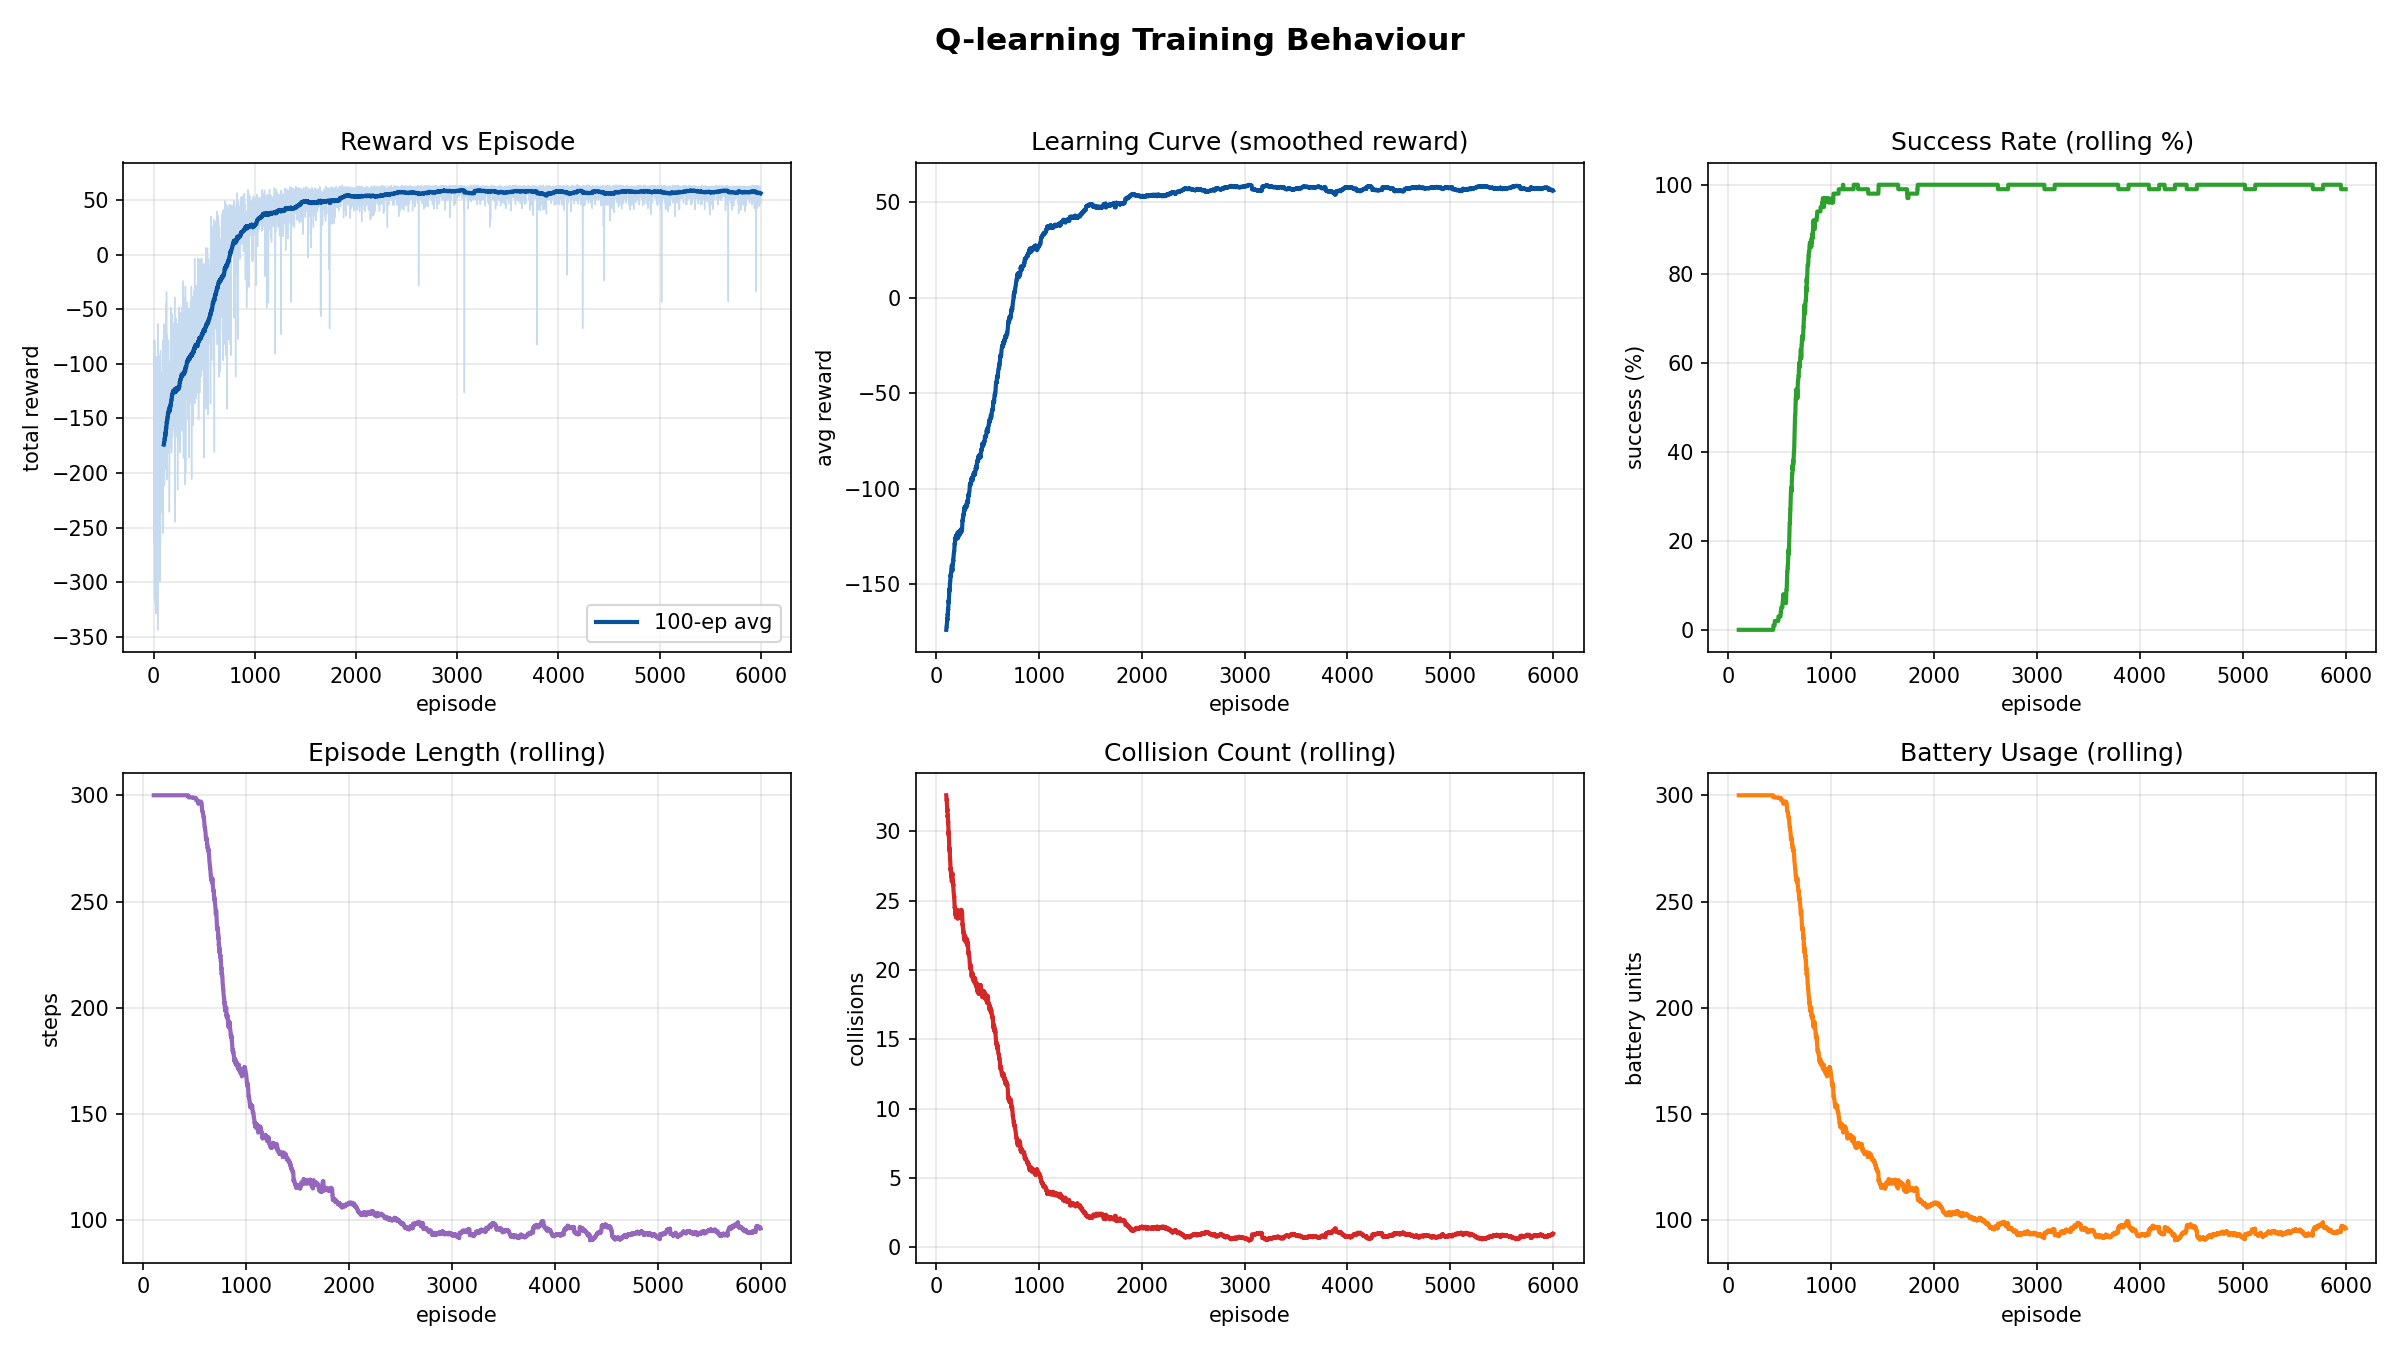
\includegraphics[width=\textwidth]{QLearning/ql_training_curves.png}
\caption{\textbf{Q-learning training behaviour} --- six diagnostic panels, all
with x-axis \emph{episode} (one full attempt at the mission).}
\end{figure}
\readhead
\begin{readlist}
  \item \textbf{Top-left --- Reward vs Episode:} the pale line is the raw
        per-episode reward (very noisy); the dark line is its \emph{100-episode
        average}. It climbs from strongly negative (random flailing) to
        positive (solving the task).
  \item \textbf{Top-middle --- Learning Curve:} just the smoothed reward, so the
        upward trend is crisp.
  \item \textbf{Top-right --- Success Rate (\%):} rolling share of episodes that
        finish the whole mission; it climbs to $100\%$.
  \item \textbf{Bottom-left --- Episode Length:} rolling number of steps per
        episode; \emph{falls} as the agent stops wandering.
  \item \textbf{Bottom-middle --- Collisions:} rolling wall-bumps per episode;
        \emph{falls} as the agent learns to avoid obstacles.
  \item \textbf{Bottom-right --- Battery Usage:} rolling energy per episode;
        falls with the shorter routes.
  \item \textbf{Take-away:} reward and success up, while length/collisions/
        battery down --- the textbook signature of successful learning.
\end{readlist}

\begin{figure}[H]
\centering
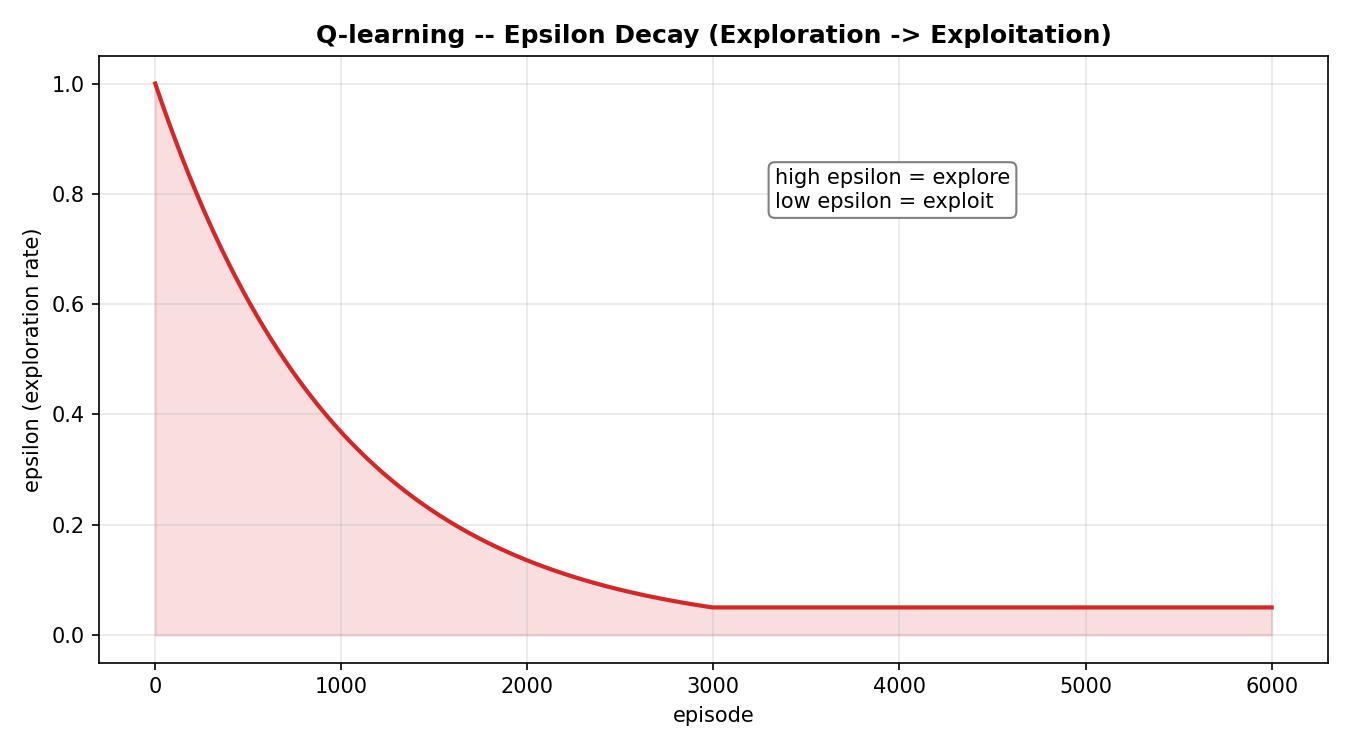
\includegraphics[width=0.72\textwidth]{QLearning/ql_epsilon_decay.png}
\caption{\textbf{$\varepsilon$ decay schedule} --- the exploration rate over
training.}
\end{figure}
\readhead
\begin{readlist}
  \item \textbf{x-axis:} episode. \textbf{y-axis:} $\varepsilon$, the chance of
        taking a \emph{random} move.
  \item The curve decays from $1.0$ (start: $100\%$ random --- pure
        exploration, since the agent knows nothing) down to a floor of $0.05$
        (mostly exploiting what it learned).
  \item \textbf{The annotation} spells it out: high $\varepsilon$ = explore,
        low $\varepsilon$ = exploit.
  \item \textbf{Take-away:} this schedule is \emph{why} the reward curve above
        can rise --- early randomness discovers good moves, later greediness
        locks them in.
\end{readlist}

\begin{figure}[H]
\centering
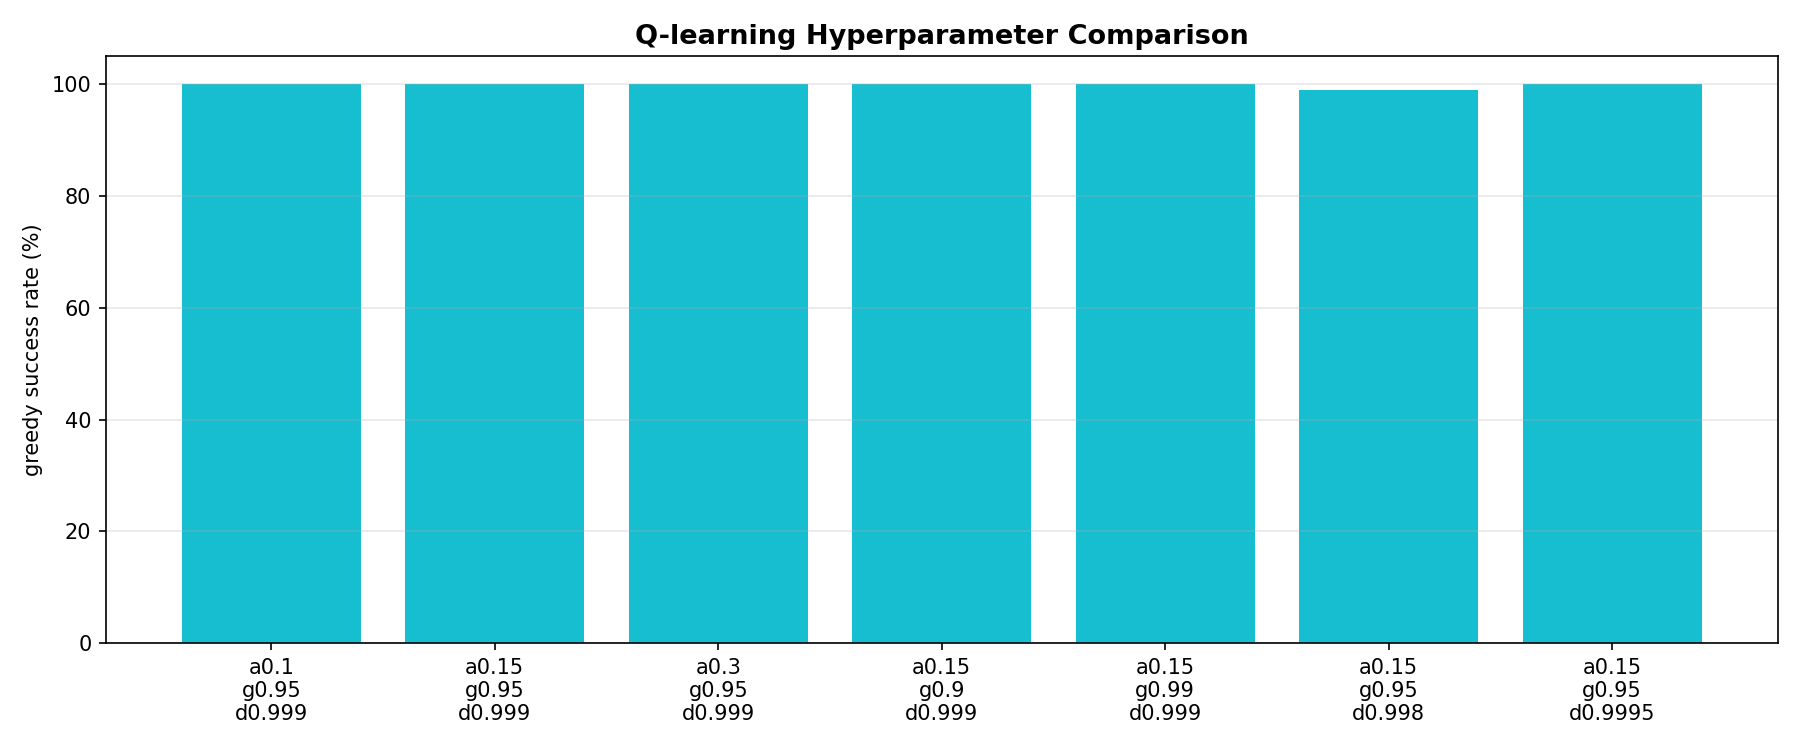
\includegraphics[width=\textwidth]{QLearning/ql_hyperparameter_comparison.png}
\caption{\textbf{Q-learning hyperparameter study} --- one bar per
configuration.}
\end{figure}
\readhead
\begin{readlist}
  \item \textbf{x-axis label} encodes the setting: \texttt{a}=$\alpha$ (learning
        rate), \texttt{g}=$\gamma$ (discount), \texttt{d}=$\varepsilon$-decay.
  \item \textbf{Bar height = greedy success rate (\%)}; here higher is better.
  \item \textbf{Take-away:} most settings reach $100\%$, but a \emph{too-fast}
        decay (agent stops exploring before it has learned enough) visibly
        lowers its bar.
\end{readlist}

% =====================================================================
\section{Value Iteration vs.\ Q-learning}
% =====================================================================
Both methods solve the identical grid and are scored the same way --- rolled
out over $200$ episodes \emph{with the $0.8/0.1/0.1$ actuator noise switched
on} --- so the comparison is strictly like-for-like.

\begin{figure}[H]
\centering
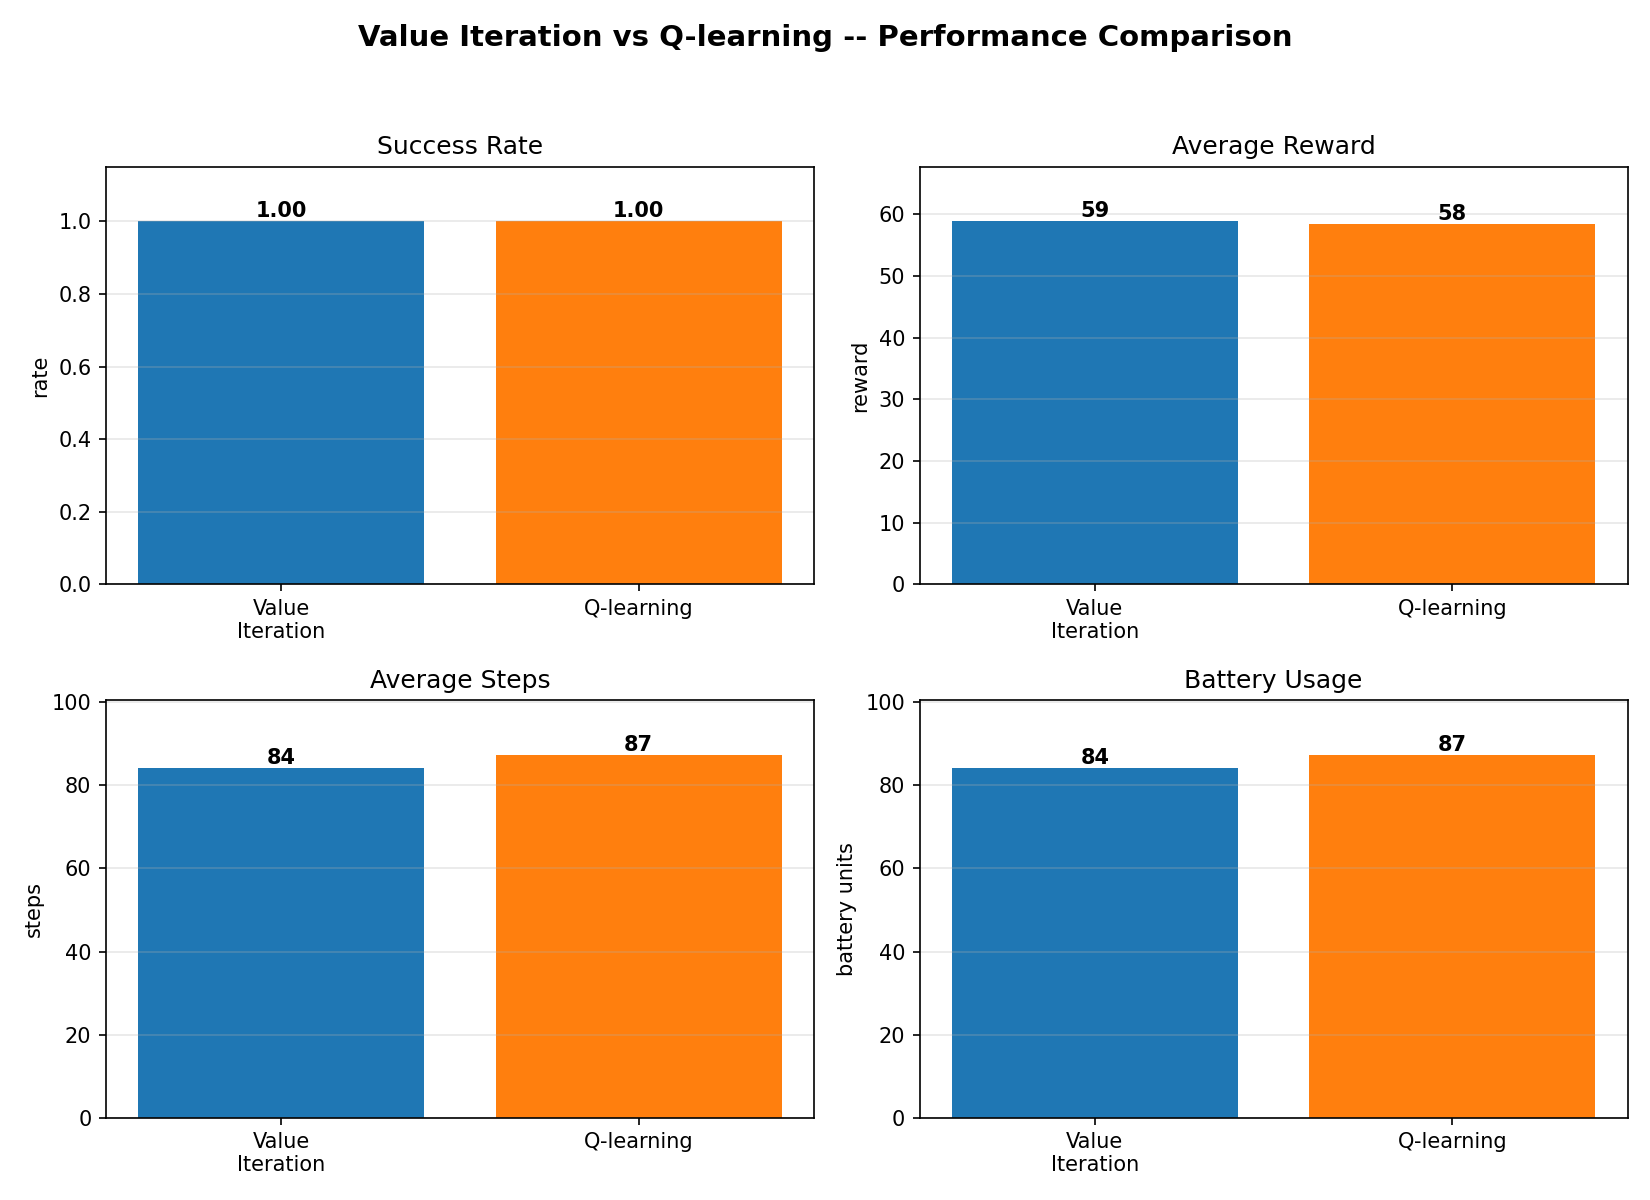
\includegraphics[width=\textwidth]{Comparison/comparison_bar.png}
\caption{\textbf{VI vs.\ Q-learning performance} --- four panels; in each, the
\emph{blue} bar is Value Iteration and the \emph{orange} bar is Q-learning.}
\label{fig:cmpbar}
\end{figure}
\readhead
\begin{readlist}
  \item \textbf{Value labels} sit on top of every bar for exact reading.
  \item \textbf{Success Rate:} both $100\%$. \textbf{Average Reward:} VI
        slightly higher (better). \textbf{Average Steps} and \textbf{Battery:}
        VI slightly lower (better) --- the small, honest cost of learning
        without a map.
  \item \textbf{Convergence} is deliberately \emph{not} a bar here, because VI
        counts Bellman \emph{iterations} while Q-learning counts training
        \emph{episodes} (different units); the like-for-like view is
        Figure~\ref{fig:convcmp}.
  \item \textbf{Take-away:} the classic \emph{model-based vs.\ model-free}
        trade-off --- VI is a touch better and far faster \emph{because} it
        already knows the map.
\end{readlist}

\begin{figure}[H]
\centering
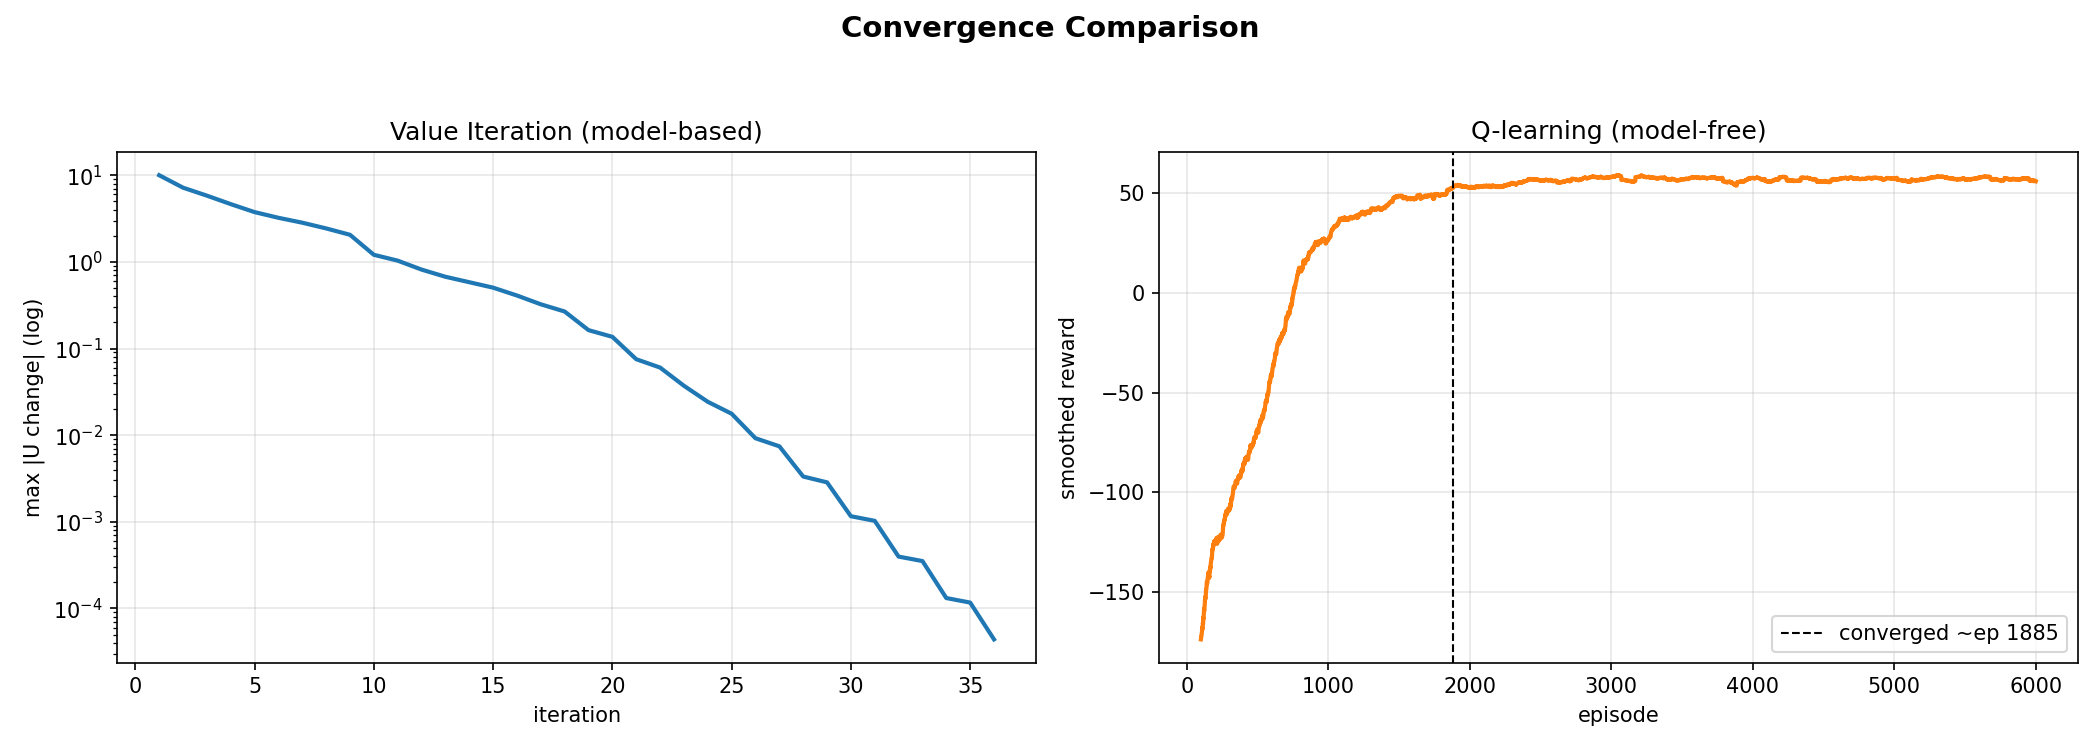
\includegraphics[width=\textwidth]{Comparison/comparison_convergence.png}
\caption{\textbf{Convergence comparison (like-for-like)} --- two panels with
\emph{different} x-units, shown separately on purpose.}
\label{fig:convcmp}
\end{figure}
\readhead
\begin{readlist}
  \item \textbf{Left --- Value Iteration:} $\max|U$ change$|$ (log axis) vs
        iteration; it plunges to the threshold in tens of iterations.
  \item \textbf{Right --- Q-learning:} smoothed reward vs episode; the dashed
        vertical line marks where it has effectively converged
        ($\sim$$1900$ episodes).
  \item They are on \emph{separate} axes because ``an iteration'' and ``an
        episode'' are not the same unit --- this is the rigorous companion to
        the mixed-unit bar in Figure~\ref{fig:cmpbar}.
  \item \textbf{Take-away:} knowing the model (left) reaches the answer in a
        fraction of the effort that learning it (right) requires.
\end{readlist}

\begin{figure}[H]
\centering
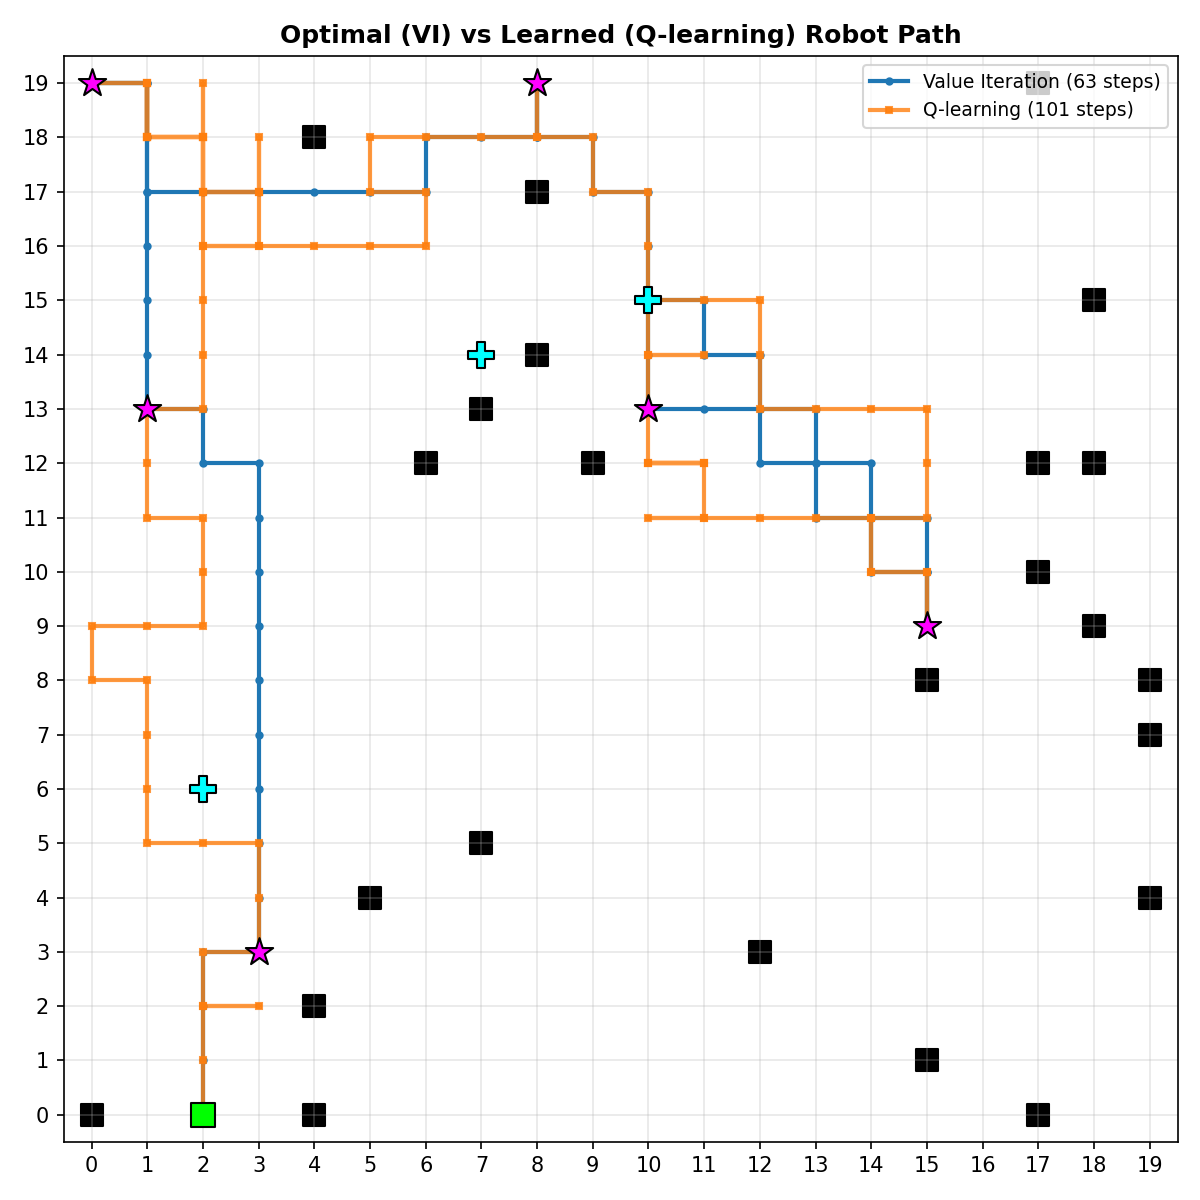
\includegraphics[width=0.62\textwidth]{Comparison/vi_vs_ql_trajectory.png}
\caption{\textbf{Optimal vs.\ learned path} --- both robots' routes drawn on
one grid.}
\end{figure}
\readhead
\begin{readlist}
  \item \textbf{Blue line with circles:} the Value-Iteration (optimal) path;
        \textbf{orange line with squares:} the Q-learning (learned) path. The
        legend gives each one's step count.
  \item Grid markers as usual: $\bigstar$ = flowers, black squares =
        obstacles, cyan ``P'' = charging, start marked on the grid.
  \item \textbf{Take-away:} both visit every flower and return to charge; the
        blue path is a little shorter --- you can literally \emph{see} the cost
        of learning without a model.
\end{readlist}

\begin{figure}[H]
\centering
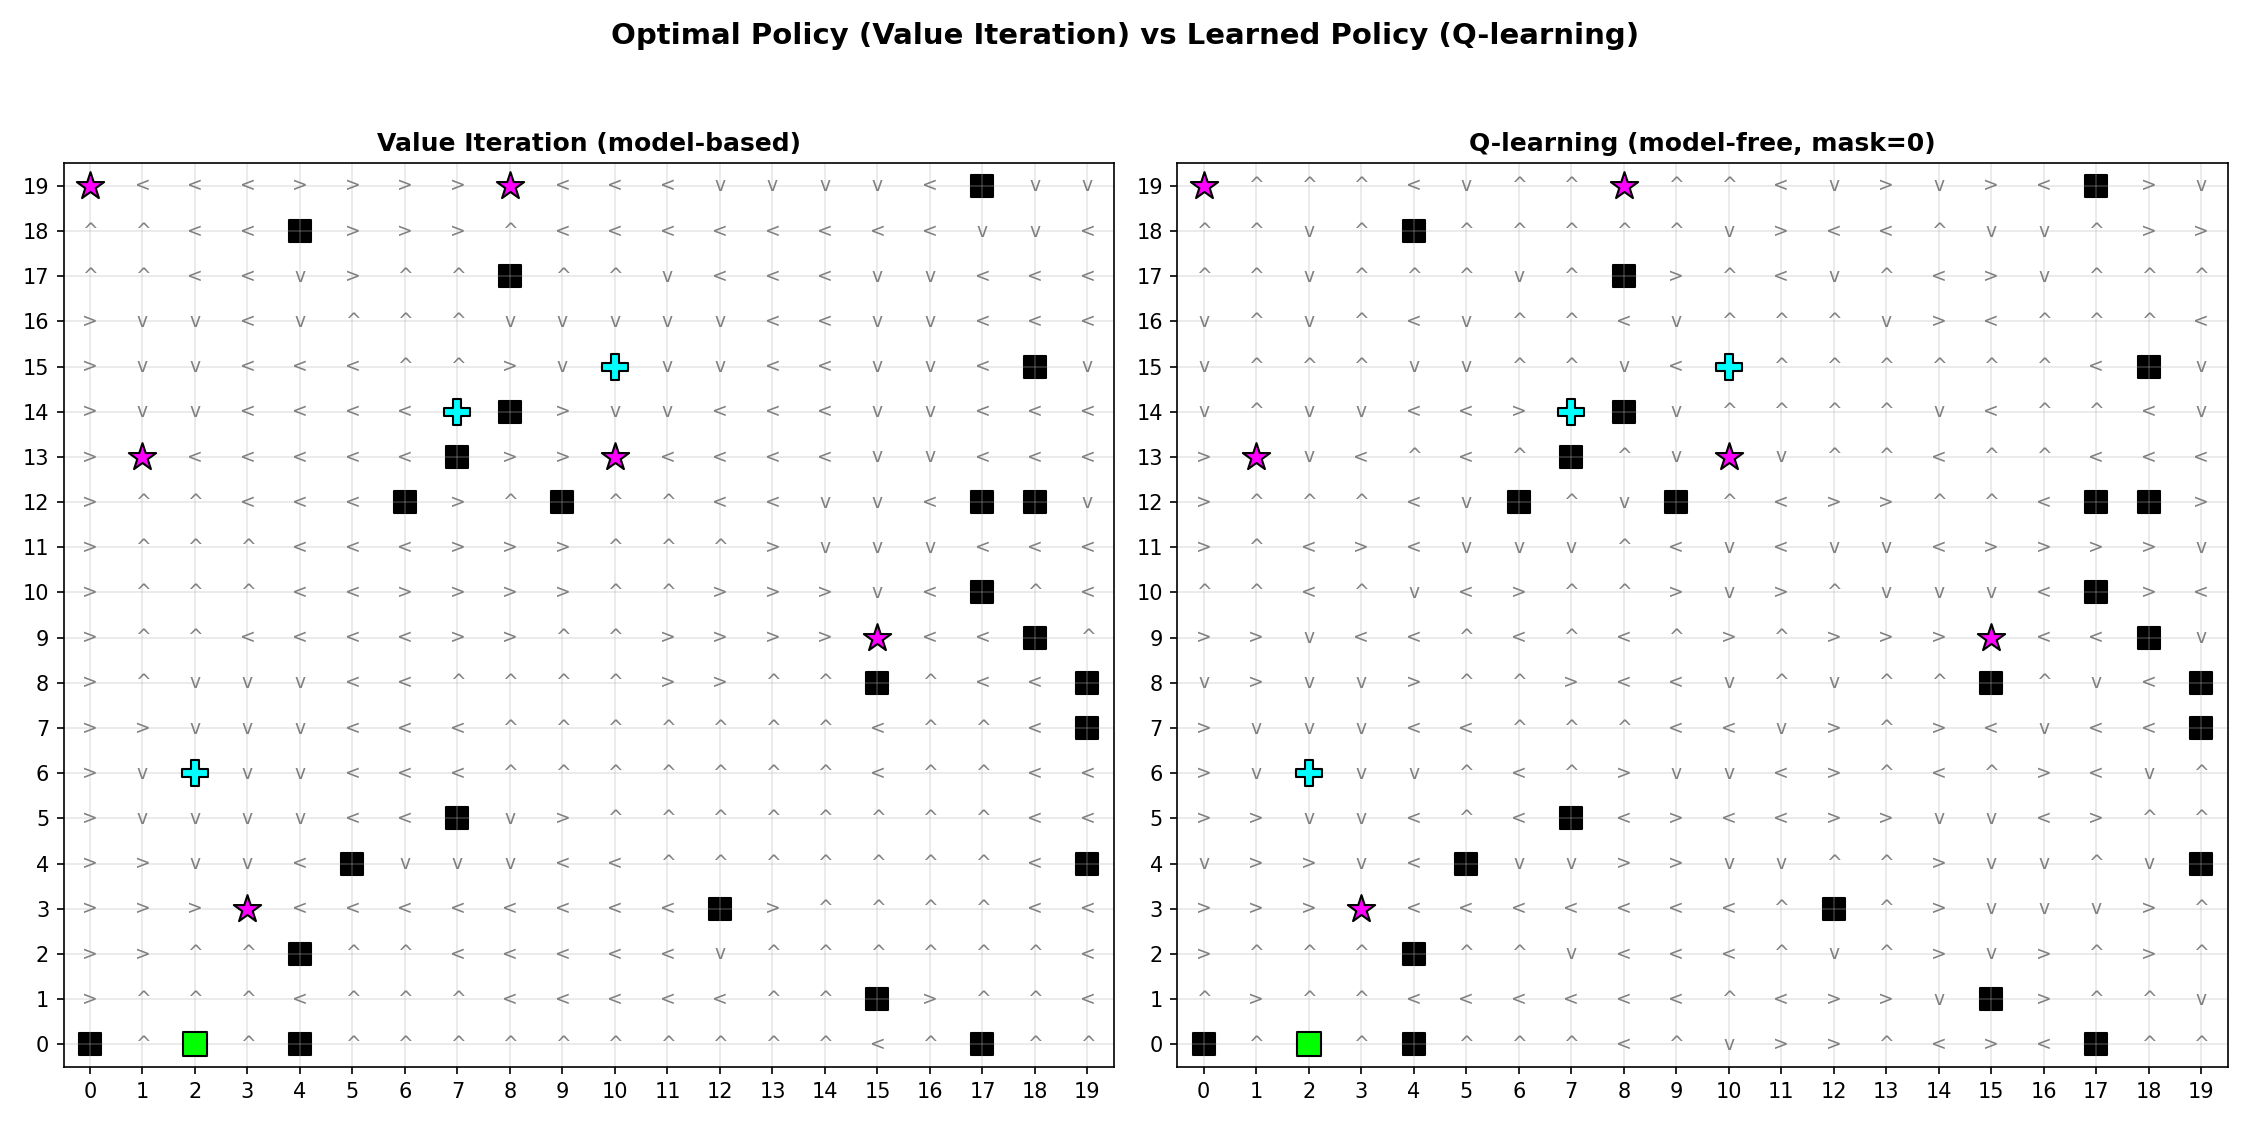
\includegraphics[width=\textwidth]{Comparison/vi_vs_ql_policy.png}
\caption{\textbf{Optimal vs.\ learned policy} --- two arrow maps side by side.}
\end{figure}
\readhead
\begin{readlist}
  \item \textbf{Left:} the Value-Iteration policy. \textbf{Right:} the
        Q-learning policy for the ``no flower collected yet'' state
        (\texttt{mask=0}).
  \item In both, a grey arrow in each cell is the best move from that cell;
        $\bigstar$/squares/``P'' mark flowers/obstacles/charging as before.
  \item \textbf{Take-away:} near the flowers the two arrow-fields point the same
        way --- model-free Q-learning \emph{rediscovered} essentially the
        optimal policy that model-based VI computed directly.
\end{readlist}

% =====================================================================
\section{Summary of Key Results}
% =====================================================================
\begin{table}[H]
\centering
\caption{Task allocation: Random vs.\ PSO vs.\ GA (identical greenhouse and
fitness). \textbf{Lower is better} for every row except the last.}
\begin{tabular}{lrrr}
\toprule
Metric & Random & PSO & GA \\
\midrule
Fitness (lower is better) & 1.77 & 1.59 & \textbf{1.43} \\
Total distance (m)        & 2663 & 2451 & \textbf{2204} \\
Energy (units)            & 266  & 245  & \textbf{220}  \\
Completion time (s)       & 282  & 267  & \textbf{255}  \\
Workload std.\ dev.       & 7.1  & 2.1  & \textbf{1.1} \\
Coverage / Utilization    & $100\%$ & $100\%$ & $100\%$ \\
\bottomrule
\end{tabular}
\end{table}

\begin{table}[H]
\centering
\caption{Navigation: Value Iteration vs.\ Q-learning (same grid-world MDP,
identical stochastic test).}
\begin{tabular}{lrr}
\toprule
Metric & Value Iteration & Q-learning \\
\midrule
Success rate       & $100\%$ & $100\%$ \\
Average reward     & 58.8    & 58.4 \\
Average steps      & 84      & 87 \\
Battery usage      & 84      & 87 \\
Execution time (s)$^{\dagger}$ & $\sim 0.05$ & $\sim 9\text{--}17$ \\
Convergence        & 36 iterations & 1885 episodes \\
\bottomrule
\end{tabular}

\vspace{2pt}
{\footnotesize $^{\dagger}$ Wall-clock time; hardware/load dependent and the
only non-reproducible metric. Reward/steps/battery are averaged over 200
test episodes \emph{under the identical $0.8/0.1/0.1$ actuator-noise model}
for \emph{both} methods (Value Iteration's optimal policy is rolled out the
same way Q-learning is tested), so the row is strictly like-for-like and
reproducible under the fixed seed. ``Convergence'' units differ (iterations
vs.\ episodes).}
\end{table}

\end{document}
